\documentclass[journal]{IEEEtran}

\usepackage{amsmath,amssymb,amsfonts,amsthm}
\usepackage{euscript}
\usepackage[latin1]{inputenc}
\usepackage[T1]{fontenc}
\usepackage{color}
\usepackage{graphicx}
\usepackage{mathrsfs}
\usepackage{algorithm}
\usepackage{algorithmic}
\usepackage{dsfont}
\usepackage[shortlabels]{enumitem}
\usepackage{multirow}
\usepackage{hhline}
\usepackage{hyperref}
\usepackage{mathpazo}
\usepackage{array}
\usepackage{bigints}

\graphicspath{{figures/}}
\def\matlab{{\sc Matlab\ }}
\def\octave{{\sc Octave}}
\renewcommand{\Re}{\operatorname{Re}}
\renewcommand{\Im}{\operatorname{Im}}


%\def\foorp{{\hfill$\spadesuit$}}
\def\foorp{{\hfill$\square$}}
\def\ds{{\displaystyle}}
\def\inv{{^{-1}}}
\def\HH{{\mathbb H}}
\def\MM{{\mathbb M}}
\def\tMM{\tilde{\mathbb M}}
\def\RR{{\mathbb R}}
\def\SS{{\mathbb S}}
\def\PP{{\mathbb P}}
\def\EE{{\mathbb E}}
\def\Pr#1{{\PP\!\left\{#1\right\}}}
\def\Ex#1{{\EE\left\{#1\right\}}}
\def\var#1{{\hbox{Var}\left\{#1\right\}}}
\def\QQ{\mathbb Q}
\def\CC{\mathbb C}
\def\ZZ{\mathbb Z}
\def\NN{\mathbb N}
\def\Id{{\mathbbm 1}}
\def\cN{\mathcal N}
\def\dd#1{\mathrm{d}#1}

\def\tX{\tilde{X}}

\def\ii{\mathrm{i}}

\def\1{\mathds{1}}

%\def\o{\overline}
\def\la{\langle}
\def\ra{\rangle}

\def\ch{{\rm ch}}
\def\sh{{\rm sh}}


\def\rf#1{(\ref{#1})}
\def\be{\begin{equation}}
\def\beq#1{\begin{equation}\label{#1}}
\def\ee{\end{equation}}
\def\bea{\begin{eqnarray}}
\def\beqa#1{\begin{eqnarray}\label{#1}}
\def\eea{\end{eqnarray}}
\def\ba{\begin{array}}
\def\ea{\end{array}}


\DeclareMathAlphabet{\mathpzc}{OT1}{pzc}{m}{it}

\def\defeq{\overset{\Delta}{=}}

\def\eg{e.g.\@}
\def\ie{i.e.\@}
\def\etal{\textit{et al.}}


\def\cA{{\mathcal A}}
\def\cB{{\mathcal B}}
\def\cC{{\mathcal C}}
\def\ccC{{\mathscr C}}
\def\cCN{{\mathcal {C\!N}}}
\def\tcC{\tilde{\mathcal C}}
\def\cD{{\mathcal D}}
\def\ccD{{\mathscr D}}
\def\cE{{\mathcal E}}
\def\cF{{\mathcal F}}
\def\ccF{{\mathscr F}}
\def\cG{{\mathcal G}}
\def\ccG{{\mathcal G}}
\def\ocF{\overline{\mathcal F}}
\def\cH{{\mathcal H}}
\def\ccH{{\mathscr H}}
\def\cJ{{\mathcal J}}
\def\ck{{\mathcal k}}
\def\cK{{\mathcal K}}
\def\cL{{\mathcal L}}
\def\ccL{{\mathscr L}}
\def\cM{{\mathcal M}}
\def\ccM{{\mathscr M}}
\def\cN{{\mathcal N}}
\def\cP{{\mathcal P}}
\def\cQ{{\mathcal Q}}
\def\ccQ{{\mathscr Q}}
\def\cR{{\mathcal R}}
\def\ccR{{\mathscr R}}
\def\cS{{\mathcal S}}
\def\ccS{{\mathscr S}}
\def\cT{{\mathcal T}}
\def\ccT{{\mathscr T}}
\def\cO{{\mathcal O}}
\def\cU{{\mathcal U}}
\def\tcU{\widetilde{\mathcal U}}
\def\cV{{\mathcal V}}
\def\tcV{\widetilde{\mathcal V}}
\def\cW{{\mathcal W}}
\def\tcW{\widetilde{\mathcal W}}
\def\cl{{\mathpzc l}}
\def\cs{{\mathpzc s}}




\def\la{{\langle}}
\def\ra{{\rangle}}
\def\qed{\hskip 6pt\vrule height6pt width5pt depth1pt}
\def\R{\RR}
\def\Z{\ZZ}
\def\sgn{\hbox{sgn}}
\def\Lone{L^1(\RR )}
\def\Ltwo{L^2(\RR )}
\def\Linf{L^\infty(\RR )}
\def\Lba{L^2(\RR\times\RR_+^* ,a^{-1}dadb)}
\def\Htwo{H^2(\RR )}
\def\lone{\ell^1(\ZZ )}
\def\ltwo{\ell^2(\ZZ )}
\def\gets{$<\!\!\! -\,$}
%\def\Id{{\bf 1}}
\def\bds{_{-\infty}^\infty}
\def\supp{\hbox{supp}}
\def\mod{{\mathrm {mod}}}
\def\modN{[\hbox{\footnotesize mod }N]}

% bold
\def\bpsi{\boldsymbol{\psi}}
\def\bPsi{\boldsymbol{\Psi}}
\def\balpha{\boldsymbol{\alpha}}
\def\bbeta{\boldsymbol{\beta}}
\def\bDelta{\boldsymbol{\Delta}}
\def\bzero{\boldsymbol{0}}
\def\blambda{\boldsymbol{\lambda}}
\def\bLambda{\boldsymbol{\Lambda}}
\def\bSigma{\boldsymbol{\Sigma}}
\def\bepsilon{\boldsymbol{\epsilon}}
\def\bgamma{\boldsymbol{\gamma}}
\def\bGamma{\boldsymbol{\Gamma}}
\def\bmu{\boldsymbol{\mu}}
\def\bnabla{\boldsymbol{\nabla}}
\def\bphi{\boldsymbol{\varphi}}
\def\bPsi{\boldsymbol{\Psi}}
\def\brho{\boldsymbol{\rho}}
\def\btheta{\boldsymbol{\theta}}
\def\bTheta{\boldsymbol{\Theta}}
\def\btau{\boldsymbol{\tau}}
\def\bxi{\boldsymbol{\xi}}
\def\bnu{\boldsymbol{\nu}}
\def\bOmega{\boldsymbol{\Omega}}

\def\ba{{\mathbf a}}
\def\bA{{\mathbf A}}
\def\bb{{\mathbf b}}
\def\bB{{\mathbf B}}
\def\bC{{\mathbf C}}
\def\bD{{\mathbf D}}
\def\be{{\mathbf e}}
\def\bE{{\mathbf E}}
\def\bff{{\mathbf f}}
\def\bF{{\mathbf F}}
\def\bg{{\mathbf g}}
\def\bG{{\mathbf G}}
\def\bh{{\mathbf h}}
\def\bH{{\mathbf H}}
\def\bI{{\mathbf I}}
\def\bJ{{\mathbf J}}
\def\bK{{\mathbf K}}
\def\bL{{\mathbf L}}
\def\bm{{\mathbf m}}
\def\bM{{\mathbf M}}
\def\bN{{\mathbf N}}
\def\bo{{\mathbf o}}
\def\bO{{\mathbf O}}
\def\bP{{\mathbf P}}
\def\bq{{\mathbf q}}
\def\bQ{{\mathbf Q}}
\def\br{{\mathbf r}}
\def\bR{{\mathbf R}}
\def\bs{{\mathbf s}}
\def\bS{{\mathbf S}}
\def\bt{{\mathbf t}}
\def\bT{{\mathbf T}}
\def\bu{{\mathbf u}}
\def\bU{{\mathbf U}}
\def\bv{{\mathbf v}}
\def\bV{{\mathbf V}}
\def\bw{{\mathbf w}}
\def\bW{{\mathbf W}}
\def\bx{{\mathbf x}}
\def\bX{{\mathbf X}}
\def\by{{\mathbf y}}
\def\bY{{\mathbf Y}}
\def\bZ{{\mathbf Z}}
\def\bz{{\mathbf z}}

% overline
\def\ox{\overline{x}}
\def\oy{\overline{y}}
\def\oz{\overline{z}}

% tilde
\def\tb{{\tilde{b}}}
\def\te{{\tilde{e}}}
\def\tf{{\tilde{f}}}
\def\tg{{\tilde{g}}}
\def\th{{\tilde{h}}}
\def\tk{{\tilde{k}}}
%\def\tt{{\tilde{t}}}
\def\tp{{\tilde{p}}}
\def\tu{{\tilde{u}}}
\def\tv{{\tilde{v}}}
\def\tx{{\tilde{x}}}
\def\ty{{\tilde{y}}}
\def\tz{{\tilde{z}}}
\def\tp{{\tilde{p}}}
\def\tq{{\tilde{q}}}

\def\tgamma{{\tilde\gamma}}
\def\tGamma{{\tilde\Gamma}}
\def\tsigma{{\tilde\sigma}}
\def\tSigma{{\tilde\Sigma}}
\def\tpi{{\tilde\pi}}
\def\tpsi{{\tilde\psi}}
\def\trho{{\tilde\rho}}
\def\tX{{\tilde{X}}}
\def\tY{{\tilde{Y}}}
\def\S{{\tilde{S}}}
\def\T{{\tilde{T}}}

% hat
\def\hb{{\hat b}}
\def\he{{\hat e}}
\def\hh{{\hat h}}
\def\hk{{\hat k}}
\def\hp{{\hat p}}
% \def\ht{{\hat t}}
\def\hu{{\hat u}}
\def\hv{{\hat v}}
\def\hw{{\hat w}}
\def\hx{{\hat x}}
\def\hy{{\hat y}}
\def\hz{{\hat z}}
\def\hLambda{{\hat \Lambda}}
\def\hDelta{{\hat \delta}}
\def\hlambda{{\hat \lambda}}
\def\hdelta{{\hat \delta}}
\def\halpha{{\hat \alpha}}
\def\hbeta{{\hat \beta}}
\def\htheta{{\hat \theta}}
\def\hsigma{{\hat \sigma}}


% vectors (underline)
\def\a{{\underline{a}}}
\def\e{{\underline{e}}}
\def\h{{\underline{h}}}
\def\k{{\underline{k}}}
\def\m{{\underline{m}}}
\def\t{{\underline{t}}}
\def\u{{\underline{u}}}
\def\w{{\underline{w}}}
\def\x{{\underline{x}}}
\def\y{{\underline{y}}}
\def\z{{\underline{z}}}

\def\X{{\underline{X}}}
\def\Y{{\underline{Y}}}
\def\S{{\underline{S}}}
\def\T{{\underline{T}}}

\def\Om{{\underline{\Omega}}}

\def\ual{{\underline\alpha}}
\def\ubet{{\underline\beta}}
%
% Matrices
\def\A{{\underline{\underline{A}}}}
\def\RX{{\underline{\underline{R}}_X}}

%
% Algebraic quantities
\def\rg#1{{\hbox{rg}\left(#1\right)}}

\def\fs{f_{\mathsf s}}


\title{An Efficient Forecasting Approach\\ to Reduce Boundary Effects in Real-Time Time-Frequency Analysis}

\author{Adrien~Meynard, %~\IEEEmembership{Member,~IEEE,}
        Hau-Tieng~Wu
\thanks{A. Meynard is with the Department
of Mathematics, Duke University, Durham,
NC, 27708 USA.

H.-T. Wu is with the Department of Mathematics and Department of Statistical Science, Duke University, Durham, NC, 27708 USA; Mathematics Division, National Center for Theoretical Sciences, Taipei, Taiwan.
 
A. Meynard is the corresponding author (e-mail: adrien.meynard@duke.edu).
}}

\newtheorem{remark}{Remark}
\newtheorem{lemma}{Lemma}
\newtheorem{theorem}{Theorem}

\begin{document}

\maketitle

\begin{abstract}
Time-frequency (TF) representations of time series are intrinsically subject to the boundary effects. As a result, the structures of signals that are highlighted by the representations are garbled when approaching the boundaries of the TF domain. In this paper, for the purpose of real-time TF information acquisition of nonstationary oscillatory time series, we propose a numerically efficient approach for the reduction of such boundary effects. The solution relies on an extension of the analyzed signal obtained by a forecasting technique. In the case of the study of a class of locally oscillating signals, we provide a theoretical guarantee of the performance of our approach. Following a numerical verification of the algorithmic performance of our approach, we validate it by implementing it on biomedical signals.
\end{abstract}

\begin{IEEEkeywords}
Boundary effects, time-frequency, forecasting, nonstationarity
\end{IEEEkeywords}

\section{Introduction}
\label{se:introduction}
\IEEEPARstart{I}{n} any digital acquisition system, the study and the interpretation of the measured signals generally require an analysis tool, which enables researchers to point out the useful characteristics of the signal. The need for signal analysis arises from various signals, ranging from audio~\cite{Stowell18computational,Muller11signal}, mechanical~\cite{Peng02vibration}, or biomedical signals~\cite{Akay96detection}. For instance, biomedical signals, such as photoplethysmogram (PPG), contain several characteristics, including respiratory rate or blood pressure, that cannot be interpreted from its run-sequence plot in the time domain. An analysis tool would make possible the extraction of these useful characteristics. 

Usually, the measured signals exhibit nonstationary behavior, and the observed quantities might be interfered with by transient phenomena that can vary rapidly and irregularly. In this paper, we focus on oscillatory time series. These signals might, for example, oscillate fast with large amplitudes at one moment, and then oscillate slowly with small amplitudes at the next moment. In order to adapt the analysis to nonstationarities, local spectral analysis is generally performed~\cite{Stoica05spectral,Matz97generalized}. The short-time Fourier transform~\cite{Grochenig01foundations} (STFT), a typical tool built for this purpose, enables the determination of the local frequency content of a nonstationary signal.

Windowing is a common method for performing local analysis. Among many others, STFT~\cite{Flandrin:1999}, continuous wavelet transform (CWT)~\cite{Da1992}, synchrosqueezing transform (SST) \cite{Daubechies11synchrosqueezed}, and reassignment~\cite{Auger13time} (RS) are representations that fall back on the use of an analysis window. Let $x:I\to\RR$ denote the observed signal, where $I$ denotes the finite interval where the signal is measured. Let $g_s:\RR\to\RR$ denote the analysis window, where $s$ is a shape parameter. The support of $g_s$ is localized around the origin and is small with respect to $|I|$. The translation operator is $T_\tau$ defined as:
\[
T_\tau f = f(t-\tau)\ ,\quad \forall\ f:\RR\to\RR\ .
\]
Then, the local analysis of $x$ around the instant $\tau\in I$ rely on the evaluation of the following inner product:
\begin{equation}
V_x(s,\tau) = \langle x, T_\tau g_s \rangle_I \ .
\label{eq:windowing}
\end{equation}
A major shortcoming of this technique occurs when analyzing the signal $x$ {\em near the boundaries} of the interval $I$. Clearly, at these points, half of the information is missing. Consequently, the results of the inner product~\eqref{eq:windowing} are distorted. This phenomenon is usually understood as the \emph{boundary effect}. The result of the SST of a PPG is shown in the lower-left corner of Fig.~\ref{fig:ex.intro} (see section~\ref{ssse:ppg} for a comprehensive description). The distortion resulting from boundary effects is clearly visible on the right side of this representation. Indeed, while in the major left part of the image, clear lines stand out, they become blurred as they approach the right boundary of the image. Therefore, estimations of signal characteristics, like instantaneous frequencies~\cite{Delprat92asymptotic} or amplitudes, from this TF representation appear to be imprecisely determinable (or even likely to fail) in the vicinity of the boundaries. Moreover, this boundary effect would unavoidably limit applying these window-based TF analysis tools for real-time analysis purposes. It is thus desirable to have a solution to eliminating the boundary effects.

\begin{figure}
\centering
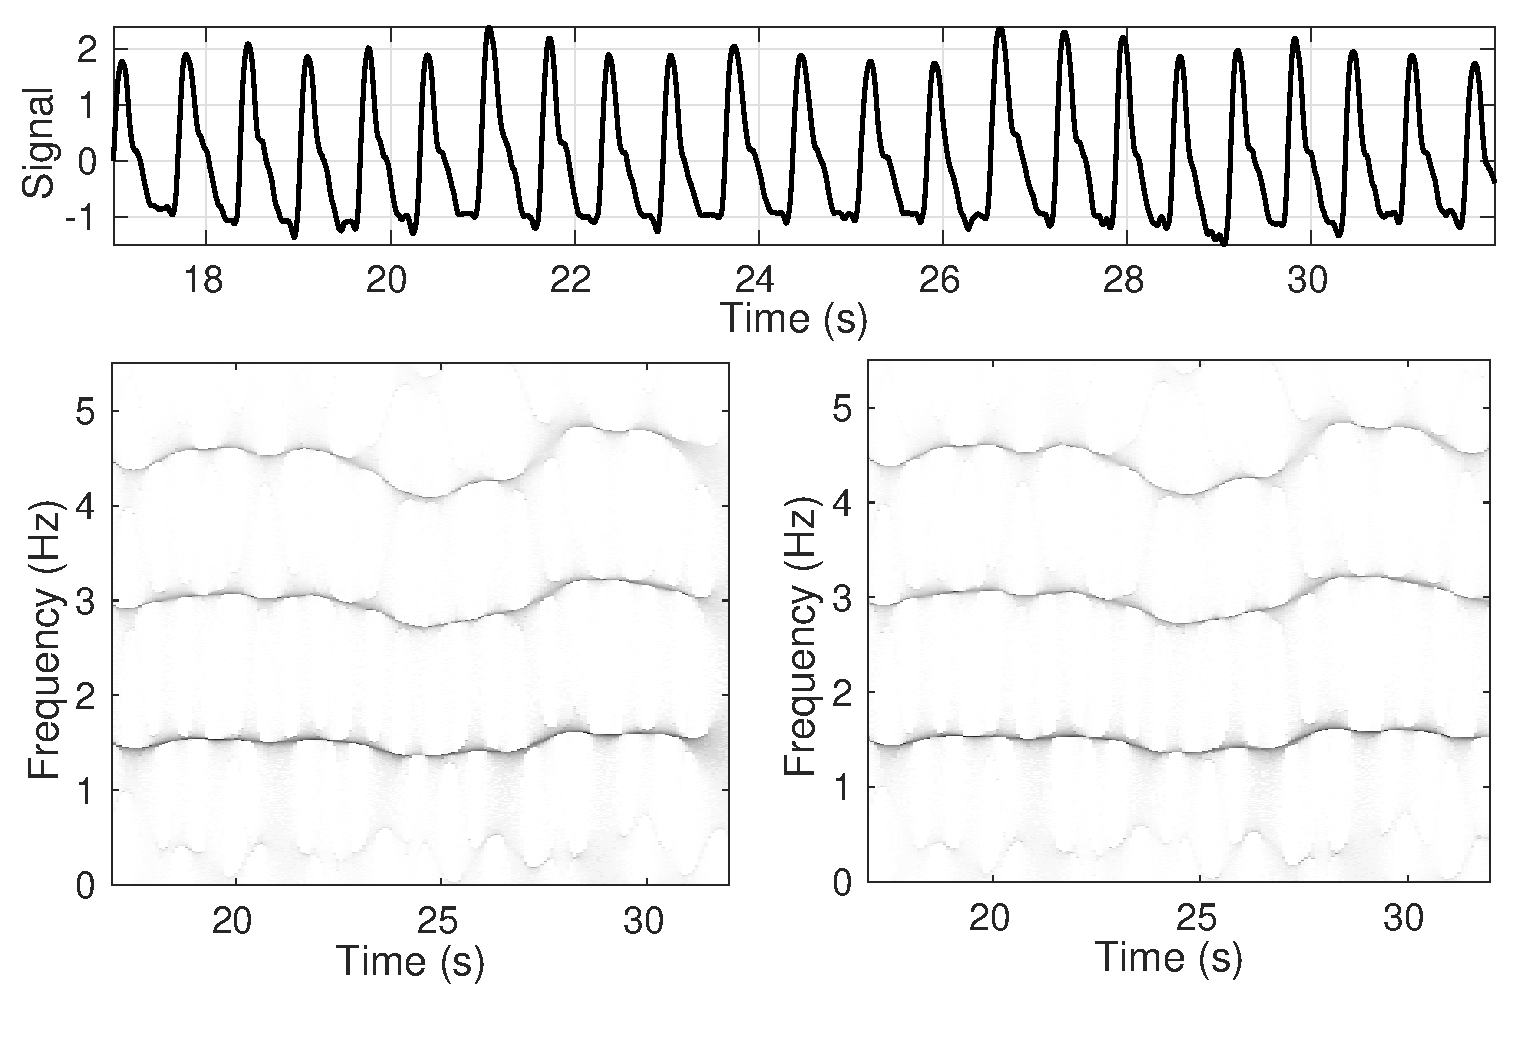
\includegraphics[width=.48\textwidth]{PPGsig.eps}
%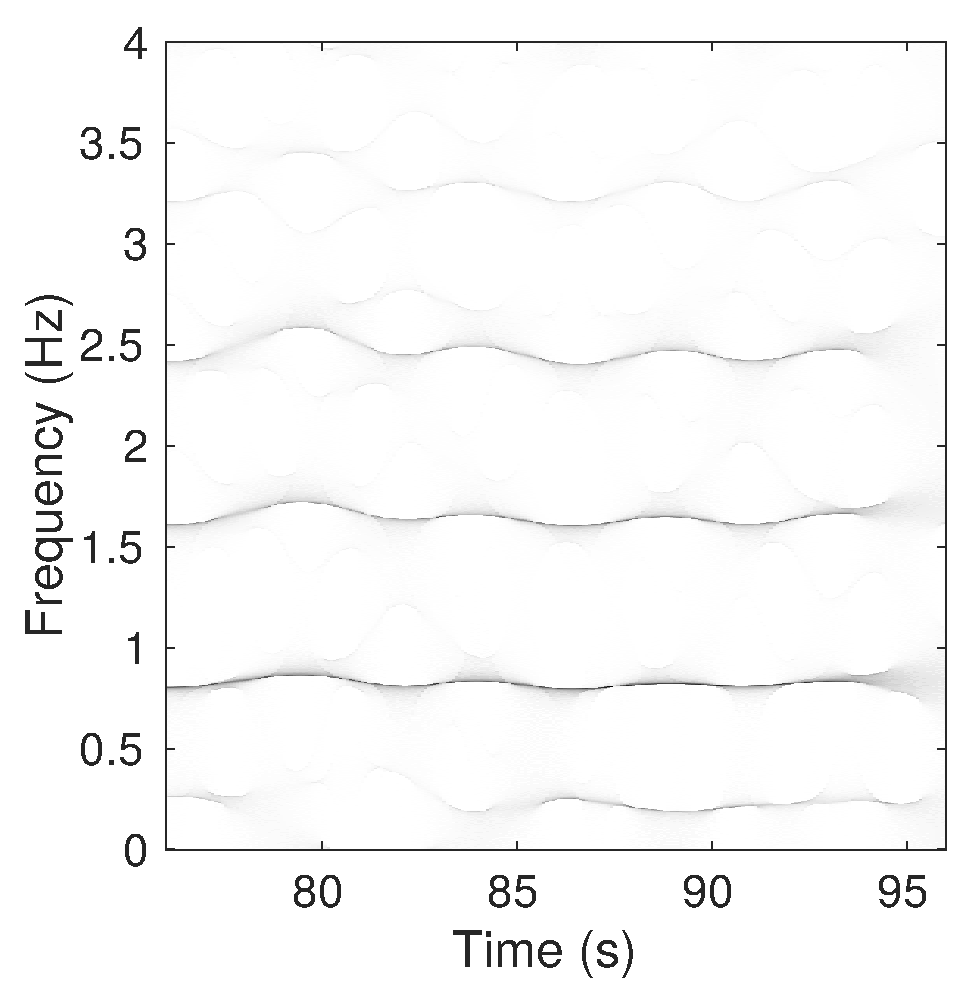
\includegraphics[width=.24\textwidth]{zoomSSTintro.eps}
%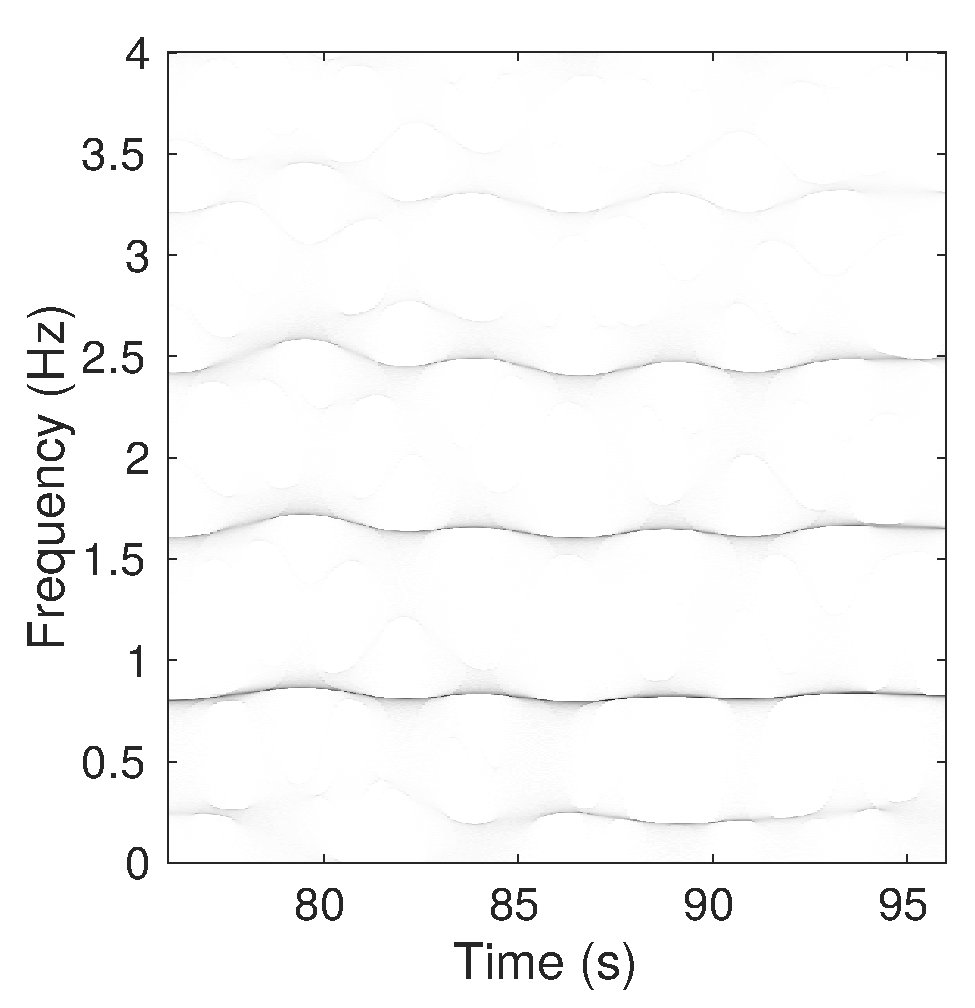
\includegraphics[width=.24\textwidth]{zoomSSTBoundEffRed.eps}
\caption{A segment of PPG signal (top) and the right boundary of a TF representation determined by the SST without extension (bottom left), and the right boundary of a TF representation determined by the SST with the proposed boundary effect reduction algorithm by forecasting (bottom right). The window length for the SST is 12~seconds.}
\label{fig:ex.intro}
\end{figure}

Attempts to minimize the boundary effects generally consists in softening the discontinuity on signal edges. Usually, the approaches can be classified into two main classes, choosing a proper analysis window and extending/forecasting the signal. In the first class, judicious choice of analysis window whose support does not interfere with the boundary points can minimize the occurrence of aberrant patterns near the boundaries of the TF plane, for instance, \cite{Chui92wavelets,Depczynski99fast}. Due to the specific relationship between the chosen analysis windows and the TF analysis tool, these techniques do not make it possible to reduce the boundary effects of all TF representations. 
%
Another natural idea, the second class, consists of carrying out a preliminary step of extending, or forecasting, the signal beyond its boundaries. Due to its flexibility, various forecasting schemes have been proposed. For example, there exist simple extension schemes that do not take into account the dynamical behavior of the signal, such as zero-padding, periodic extension, symmetric extension~\cite{Kharitonenko02wavelet,Chen95symmetric}, or polynomial extrapolation~\cite{Williams97discrete}. 
%
There exist extension schemes based on physically relevant dynamical models, such as the Extended Dynamic Mode Decomposition~\cite{Williams15data} (EDMD) and the Gaussian process regression~\cite{Rasmussen06gaussian,Roberts13Gaussian} (GPR).
% 
{\color{red}
In speech processing, dynamic mode predictors have also been proposed~\cite{Vargas11speech} to forecast signals falling into the so-called \textit{source--filter} model. This gradient-based technique rely on the shadowing approach proposed in~\cite{Grebogi90shadowing}.
} 
%
There also exist extension schemes based on stochastic models, such as the Trigonometric, Box-Cox transformation, ARMA errors, Trend and Seasonal components (TBATS) algorithm~\cite{DeLivera11forecasting}, the dynamic linear models \cite{west2006bayesian}. 
%
In the physically relevant dynamical models, the oscillation or trend, are usually modeled as the mean of a stochastic process, while in the stochastic models, the oscillation or trend are modeled by the covariance structure of the stochastic process. 
It is also possible to consider polynomial regression~\cite{fan1996local} or modeling the mean by splines~\cite{hall2005theory}, kernel functions~\cite{chang2010training}, and wavelets~\cite{marron1998exact}, or nonparametric regression~\cite{fan1996local}, to estimate the mean function before forecasting the signal. Neural network models, such as the long short-term memory model~\cite{vlachas2018data}, is another approach. 
%
The above list is far from exhaustive, and we refer readers with interest to \cite{hyndman2018forecasting} for a friendly monograph on the general forecasting topic. 
%
While the model-based extension scheme gives better-extended signals than those simple extension without dynamical models, they generally have a great computational cost. 

In this paper, we propose a fast extension algorithm based on a simple dynamical model that optimizes the trade-off between the extension quality and the computational cost, so that the real-time analysis can be achieved. The algorithm is composed of two steps.
\begin{enumerate}
\item \emph{Extend the signal by forecasting it.} The aim is to use a simple dynamic model to predict the values taken by the measured signal outside the measurement interval. Then, once this operation is done, we have access to an extended signal defined on a larger interval $I_\Delta$, where $\Delta$ denotes the size of the extension on both boundaries of $I$.
\item \emph{Run the local analysis tool on the extended signal.} Assuming that the support of the analysis window is smaller than $2\Delta$, the local analysis near the boundary of $I$ is now possible without lack of information thanks to knowledge brought by the extension. 
\end{enumerate}

Thus, assuming that the quality of the extension step is sufficient, the analysis results obtained that way will be less sensitive to the boundary effects than the result of the analysis tool applied directly to the nonextended signal. We claim and prove that forecasting oscillatory signals based on the simple dynamical model combined with the simple least square approach is sufficient for reducing the boundary effects for the TF analysis, or other kernel-based analysis. To our knowledge, such theoretical analysis does not exist in the literature. See the bottom right of Fig.~\ref{fig:ex.intro} for a snapshot of the result. The main benefit of this simple approach is a numerically efficient solution with a theoretical guarantee for real-time analysis purposes. 

The paper is organized in the following way. In section~\ref{se:algo}, we provide an extension method based on a linear dynamic model. We derive the corresponding algorithm for boundary effects reduction. In section~\ref{se:theoretical}, we show that the dynamic model we consider is sufficient to extend signals takings the form of sums of sine waves. An evaluation of the theoretical performance of our algorithm on a class of signals, the sums of sine waves, is given in section~\ref{se:theoretical}. In section~\ref{se:results}, we compare our extension method with more sophisticated methods such as EDMD, GPR, or TBATS. We show that our algorithm gives fast results of reasonable quality. Finally, we evaluate the performance of our boundary effects reduction algorithm on biomedical signals, such as respiratory signals, and compare it to the theoretical results. 

\section{Algorithm}
\label{se:algo}
As explained above, the algorithm for the reduction of boundary effects on time-frequency representations relies on two steps. These ones are detailed in the current section.

\subsection{Forecasting}

Let $x:\RR\to\RR$ denote a continuous-time signal. In this work, we consider a finite-length discretization of that one. Thus, the sampled signal $\bx$, whose length is denoted by $N$, is such that
\[
\bx[n] = x\left(\frac{n}{\fs}\right)\ ,\quad \forall n\in\{0,\ldots,N-1\}\ , 
\]
where $\fs$ denotes the sampling frequency. 

\paragraph{Notations} 
Let $M$ and $K$ be two integers such that $M<N$ and $K+M<N$. Then, for all $k\in\{0,\ldots,K-1\}$, we extract from $\bx\in\RR^N$ the sub-signal $\bx_k\in\RR^M$ given by:
\begin{equation}
\bx_k = 
\begin{pmatrix}
\bx[N-K+(k-1)-(M-1)] \\
\vdots \\
\bx[N-K+(k-1)]
\end{pmatrix}\ .
\label{eq:xk}
\end{equation} 
These sub-signals are gathered into the matrix $\bX\in\RR^{M\times K}$ such that:
\begin{equation*}
\bX = 
\begin{pmatrix}
\bx_0 & \cdots & \bx_{K-1}
\end{pmatrix}\ .
\end{equation*}
Notice that these sub-signals are overlapping each other. Indeed, $\bx_{k+1}$ is a shifting of $\bx_k$ from one sample. We also consider the matrix $\bY\in\RR^{M\times K}$ given by:
\begin{equation*}
\bY = 
\begin{pmatrix}
\bx_1 & \cdots & \bx_{K}
\end{pmatrix}\ .
\end{equation*}

\paragraph{Dynamical model and forecasting} 
Establishing a dynamical model consists in determining the relation linking $\bY$ to $\bX$, that is finding a function $f$ so that
\[
\bY = f(\bX)\ .
\]
In a general framework, forecasting means estimating the function $f$ from the observed values taken by the signal, in order to predict its future values. For instance, the dynamic mode decomposition~\cite{Schmid10dynamic,Williams15data} allows this by setting very few additional constraints on the regularity of $f$. We will see later, in section~\ref{se:theoretical}, that it is not necessary to consider such a complex dynamic model for the study of the signals of interest to us. That is why we consider here a naive dynamical model, assuming that we have the following relation:
\begin{equation}
\bY = \bA\bX\ ,
\label{eq:dyn.model}
\end{equation}
where $\bA\in\RR^{M\times M}$. We adopt a classical strategy in the study of dynamical systems, that is the linearization of a nonlinear phenomenon. Notice that this linear dynamical model can be written equivalently in function of the sub-signals $\bx_k$, as:
\begin{equation}
\bx_{k+1} = \bA\bx_{k},\ ,\forall k\in\{0,\dots,K-1\}\ .
\end{equation}


The forecasting method consists in estimating the unknown matrix $\bA$. Indeed, let $\tilde\bA$ denotes the estimate of $\bA$, we then obtain the forecasting of the signal at time $\frac{N-1+\ell}{\fs}$ by:
\begin{equation}
\label{eq:prediction}
\tilde \bx [N-1+\ell] = \balpha^{(\ell)}\bx_{K}\ ,
\end{equation}  
where $\balpha^{(\ell)}$ denotes the last row of $\tilde\bA^\ell$, that is to say:
\begin{equation}
\balpha^{(\ell)}=\be_M^T\tilde\bA^\ell\ ,
\label{eq:alpha.l}
\end{equation}
where $\be_M$ is the vector of length $M$ given by $\be_M = \begin{pmatrix} 0 & \cdots & 0 & 1\end{pmatrix}^T$.

\paragraph{Model estimation} To estimate the matrix $\bA$, we basically implement the least square estimator. Thus, we solve the following problem:
\begin{equation}
\label{eq:ls.pb}
\tilde\bA = \arg\min_{\balpha} \cL(\bA)\ ,
\end{equation}
where the loss function $\cL$ is given by:
\[
\cL(\bA) = \|\bY-\bA\bX\|^2 = \sum_{k=0}^{K-1} \|\bx_{k+1}-\bA\bx_k\|^2.
\]
Therefore, solving the problem~\eqref{eq:ls.pb}, \ie~$\nabla \cL(\tilde\bA)=\bzero$, gives the following estimate $\tilde\bA$ of the dynamical model matrix $\bA$:
\begin{align}
\tilde\bA &= \bY\bX^T(\bX\bX^T)^{-1}\ .
\label{eq:lse}
\end{align}

\begin{remark}
This expression clearly shows that the matrix $\tilde\bA$ takes the following form:
\[
\tilde\bA =
\begin{pmatrix}
0       & 1       & 0      & \cdots & 0      \\
\vdots  & \ddots  & \ddots & \ddots & \vdots  \\
\vdots  &         & \ddots & \ddots & 0  \\
0       & \cdots  & \cdots & 0      & 1  \\
\alpha_1& \cdots  & \cdots & \cdots & \alpha_M  \\
\end{pmatrix}.
\]
Then, except the row vector $\balpha = \left(\alpha_1 \cdots\alpha_M\right)$, the matrix $\bA$ is fully determined by the dynamical model.
\end{remark}

\paragraph{Signal extension} In order to reduce the boundary effects on both "sides" of the time-frequency (or time-scale) representation, we finally construct the extended signal $\tilde\bx\in\RR^{N+2L}$ concatenating the backward prediction $\tilde\bx_{\rm bw}$, the observed signal $\bx$, and the forward prediction $\tilde\bx_{\rm fw}$. We summarize the extension step in Algorithm~\ref{alg:extension}. Notice that we handle the backward estimation using the same strategy than described above, but applying it to the reverse signal $\bx^{\rm r} = \begin{pmatrix} \bx[N-1] & \cdots & \bx[0] \end{pmatrix}^T$.

\begin{algorithm}
\caption{Signal extension. $\tilde\bx = \mathsf{SigExt}(\bx,M,K,L)$}
\label{alg:extension}
\begin{algorithmic}
\STATE {\bf Inputs}: $\bx$, $M$, $K$, $L$
\STATE 
\STATE {\bf Forward forecasting.}
\STATE \quad\textbullet\ LS estimation of the forward matrix $\tilde\bA_{\rm fw}$ via equation~\eqref{eq:lse}.
\STATE \quad\textbullet\ Forward forecasting $\tilde\bx_{\rm bw}$ obtained applying equation~\eqref{eq:prediction} with $\ell\in\{1,\ldots,L\}$.
\STATE 
\STATE {\bf Backward forecasting.}
\STATE \quad\textbullet\ Reverse signal $\bx$ to $\bx^{\rm r}$. 
\STATE \quad\textbullet\ LS estimation of the backward matrix $\tilde\bA_{\rm bw}$ via equation~\eqref{eq:lse} applied to $\bx^{\rm r}$.
\STATE \quad\textbullet\ Reversed backward forecasting $\tilde\bx_{\rm bw}^{\rm r}$ obtained applying equation~\eqref{eq:prediction} to $\bx^r$ with $\ell\in\{1,\ldots,L\}$.
\STATE \quad\textbullet\ Reverse $\tilde\bx_{\rm bw}^{\rm r}$ to obtain the estimate $\tilde\bx_{\rm bw}$.
\STATE 
\STATE {\bf Output}: Extended signal $\tilde\bx = \begin{pmatrix} \tilde\bx_{\rm bw}  & \bx & \tilde\bx_{\rm fw}\end{pmatrix}^T$.
\end{algorithmic}
\end{algorithm}

\subsection{Representation}
 
Let $\ccF_{N}:\RR^{N}\to\RR^{F\times N}$ generically denotes the time-frequency or time-scale representation we are interested in. It can be, for instance, such as short-time Fourier transform (STFT), the continuous wavelet transform (CWT), the synchrosqueezing transform (SST), or the reassignment (RS). Here, $F$ typically denotes the size of the representation along the frequency axis. Due to the boundary effects, the representation $\ccF_{N}(\bx)$ shows undesired patterns when approaching its edges.For example, the instantaneous frequencies highlighted by the SST can be blurred near that edges. To limit these phenomena, we apply the representation to the estimated extended signal $\tilde\bx$. This strategy moves the boundary effects out of the time interval $I=[0, \frac{N-1}{\fs}]$. Finally, the boundary-effects insensitive representation $\ccF_N^{\mathrm{ext}}:\RR^{N}\to\RR^{F\times N}$ of $\bx$ is given for all $\nu\in\{0,\cdots,F-1\}$, $n\in\{0,\cdots,N-1\}$ by:
\begin{equation}
\ccF_N^{\mathrm{ext}}(\bx)[\nu,n] = \ccF_{N+2L}(\tilde \bx)[\nu,L+n]\ .
\label{eq:restriction}
\end{equation}
This amounts to restricting the representation $\ccF_{N+2L}(\tilde \bx)$ to the original measurement interval of $\bx$. For the sake of simplicity, we denotes the restriction operator by $\cR$, where $\cR:\RR^{F\times (N+2L)}\to\RR^{F\times N}$. Consequently, we have:
\begin{equation*}
\ccF_N^{\mathrm{ext}}(\bx) = \cR\left( \ccF_{N+2L}(\tilde \bx) \right) \ .
\end{equation*}

\subsection{Global algorithm}
Finally, the global procedure we implement to reduce boundary effects on windowing-based representations is summarized by the pseudo-code of Algorithm~\ref{alg:boundary}.

\begin{algorithm}
\caption{Tackling boundary effects. $\bF_\bx = \mathsf{BoundEffRed(}\bx,M,K,L,\ccF)$}
\label{alg:boundary}
\begin{algorithmic}
\STATE {\bf Inputs}: $\bx$, $M$, $K$, $L$, $\ccF$
\STATE 
\STATE {\bf Forecasting step.}
\STATE \quad\textbullet\ Signal extension: $\tilde\bx = \mathrm{SigExt}(\bx)$.
\STATE 
\STATE {\bf Representation step.}
\STATE \quad\textbullet\ Representation evaluation: $\ccF_{N+2L}(\tilde\bx)$.
\STATE \quad\textbullet\ Restriction of $\ccF_{N+2L}(\tilde\bx)$ to the central time interval (see~\eqref{eq:restriction}) to obtain $\bF_\bx=\ccF_N^{\mathrm{ext}}(\bx)$.
\STATE 
\STATE {\bf Output}: Signal representation $\bF_\bx$
\end{algorithmic}
\end{algorithm}


\section{Theoretical Performance}
\label{se:theoretical}
\subsection{Signal Model}
We model the deterministic part of the observed signal as a multicomponent harmonic signal; that is, a sum of sine waves:
\begin{equation}
\bz[n]=\sum_{j=1}^J\Omega_j\cos\left(2\pi f_j \frac{n}{\fs} + \varphi_j\right)\ ,
\label{eq:sum.sine}
\end{equation}
where $J$ denotes the number of components, $\Omega_j>0$ the amplitude of the $j$-th component, $f_j$ its frequency, and $\varphi_j\in[0,2\pi)$ its initial phase.
%
For the sake of simplicity, we make an additional assumption on the frequencies of each component. We assume that for all $j\in\{1,\dots,J\}$:
\begin{equation}
\exists\, p_j,p_j'\in\NN^*: \quad f_j = \dfrac{p_j}{M}\fs = \dfrac{p'_j}{K}\fs\ .
\end{equation}


In addition, the observed signal is assumed to be corrupted by an additive Gaussian white noise. Therefore, the measured discrete signal $\bx$ is written as:
\begin{equation}
\bx = \bz + \sigma\bw\ ,
\label{eq:model.noise}
\end{equation}
where $\bz$ follows model~\eqref{eq:sum.sine}, $\bw$ is a Gaussian white noise, whose variance is normalized to one, and $\sigma>0$. Clearly, $\sigma^2$ denotes the variance of the additive noise $\sigma\bw$.


\subsection{Forecasting Error}
On the forecasting interval, we decompose the estimated signal $\tilde\bx$ as follows:
\begin{equation}
\tilde \bx[n] = \bz[n] + \bepsilon[n]\ ,
\label{eq:forecasting.error}
\end{equation}
where $\bepsilon$ is the forecasting error. When $n\in I=\{0,\dots,N-1\}$, this error contains only the measurement noise, that is $\bepsilon[n]=\sigma\bw[n]$. Outside the interval $I$, the importance of the forecasting error $\bepsilon$ is also affected by the loss of information resulting from the linearization of the dynamical model we consider in~\eqref{eq:dyn.model}. To evaluate the actual behavior of the forward forecasting error $\bepsilon[n]$ when $n\geq N$, we determine its first two moments.
\begin{enumerate}
\item 
The mean, or estimation bias, is such that: 
\begin{align}
\bmu[n]&\defeq\EE\{\bepsilon[n]\} 
=\EE\{\tilde\bx[n]\} - \bz[n]\ .\label{eq:defn:bias0}
\end{align}
Given the forecasting strategy, we have $\bmu[n]=0$ when $n\in I$ and
\begin{equation}
\bmu[n]= \EE\{\balpha^{(n-N+1)}\}\bz_{K} + \sigma\EE\{\balpha^{(n-N+1)}\bw_{K}\} - \bz[n]
\label{eq:bias0}
\end{equation}
when $n\geq N$.
\item 
The covariance is given by:
\begin{align*}
\bgamma[n,n'] &\defeq \EE\{\left(\bepsilon[n]-\bmu[n]\right)\left(\bepsilon[n']-\bmu[n']\right)\}\\
&= \EE\{\tilde\bx[n]\tilde\bx[n']\}-\bz[n]\bz[n'] -\bmu[n]\bz[n'] \\
&\hspace{15pt} - \bmu[n']\bz[n] -\bmu[n]\bmu[n']\ .
\end{align*}
Thus by definition of the noise, we have $\bgamma[n,n'] =\sigma^2\delta_{n,n'}$ when $(n,n')\in I^2$. When $n\geq N$, let us denote $\ell=n-N+1$. Then, we have two cases.
\begin{enumerate}[label=(\roman*)]
\item If $n'\in I$:
\begin{equation}
\bgamma[n,n'] = \sigma\EE\{\bw[n']\balpha^{(\ell)}\}\bz_K + \sigma^2\EE\{\bw[n']\balpha^{(\ell)}\bw_K\}\ .
\label{eq:cov00}
\end{equation}
\item If $n'=N-1+\lambda\geq N$:
\begin{align}
\nonumber
\hspace{-6pt}\bgamma[n,n'] &= \bz_K^T\EE\left\{{\balpha^{(\ell)}}^T\balpha^{(\lambda)}\right\}\bz_K + \sigma\EE\{\balpha^{(\ell)}\bw_K\balpha^{(\lambda)}\}\bz_K \\
\nonumber
&\hspace{-3pt} + \sigma\EE\{\balpha^{(\lambda)}\bw_K\balpha^{(\ell)}\}\bz_K + \sigma^2\EE\{\balpha^{(\ell)}\bw_K\balpha^{(\lambda)}\bw_K\}  \\
&\hspace{-3pt} -\!\bz[n]\bz[n']-\!\bz[n]\bmu[n']-\!\bz[n]\bmu[n'] -\! \bmu[n]\bmu[n']\,.
\label{eq:cov01}
\end{align}
\end{enumerate}
Besides, we recall that $\bgamma[n,n']=\bgamma[n',n]$.
\end{enumerate}

In Theorem~\ref{th:error}, we specify the asymptotic behavior of the forecasting bias and covariance when the dataset size $K$ is great.
\begin{theorem}
\label{th:error}
Let $\bx\in\RR^N$ be a discrete-time random signal following model~\eqref{eq:model.noise}. Let $\tilde\bx$ denotes its forecasting, obtained using the extension Algorithm~\ref{alg:extension}. Let $n\geq N$ be a sample index. Then, the first-order moment of the forecasting error $\epsilon[n]$ in~\eqref{eq:forecasting.error} defined in \eqref{eq:defn:bias0} satisfies
\begin{equation}
\left|\bmu[n]\right| \leq a^{(n)}_0\sigma^2 + \dfrac1K \left( \dfrac{a^{(n)}_1}{\sigma^2} + a^{(n)}_2 \right) + o\left( \dfrac1K \right)
\label{eq:mean.error}
\end{equation}
as $K\to\infty$, where $a^{(n)}_0$, $a^{(n)}_1$, and $a^{(n)}_2$ are positive quantities, independent of $K$ and $\sigma$.
Its second-order moment $\bgamma[n,n']$ satisfies the following approximation equations:
\begin{enumerate}[label=(\roman*)]
\item if $n'\in I=\{0,\ldots,N-1\}$:
\begin{equation}
\left|\bgamma[n,n']\right|\leq b^{(n,n')}_0\sigma^2 + \!\dfrac1K\! \left( b^{(n,n')}_1\! + b^{(n,n')}_2\sigma^2 \! \right) + o\!\left( \!\dfrac1K \!\right),
\label{eq:cov.error.1}
\end{equation}
as $K\to\infty$, where $b^{(n,n')}_0$, $b^{(n,n')}_1$, and $b^{(n,n')}_2$ are positive quantities, independent of $K$ and $\sigma$;
\item if $n'\geq N$:
\begin{align}
\nonumber
\left|\bgamma[n,n']\right| &\leq c^{(n,n')}_0\sigma^2 \\
&\hspace{10pt} + \!\dfrac1K\! \left(\! \dfrac{c^{(n,n')}_1}{\sigma^2} + c^{(n,n')}_2 + c^{(n,n')}_3\sigma^2 \right) + o\!\left( \!\dfrac1K \!\right)
\label{eq:cov.error.2}
\end{align}
as $K\to\infty$, where $c^{(n,n')}_0$, $c^{(n,n')}_1$, $c^{(n,n')}_2$ and $c^{(n,n')}_3$ are positive quantities, independent of $K$ and $\sigma$.
\end{enumerate}
\end{theorem}

\begin{proof}
See the Supplementary Material. The proof is mainly based on Taylor expansions of the forecasting error. Nonoptimal values of $a^{(n)}_0$, $a^{(n)}_1$,\dots, $b^{(n,n')}_0$,\dots, $c^{(n,n')}_3$ are also provided in the proof. 
\end{proof}
%The Isserlis' theorem~\cite{Isserlis16formula}, which provides a formula for the computation of higher-order moments of Gaussian random variables.

The foracasting bias and covariance asymptotically depend linearly on the ratio $\frac{1}{K}$. This shows the need to use a sufficiently large dataset to obtain an accurate forecast. Ideally when $K\to\infty$, the forecasting error would behave like the measurement noise $\sigma\bw$, \ie~a zero-mean white noise whose variance is of the order of $\sigma^2$. However, Theorem~\ref{th:error} shows that the estimator may remain asymptotically biased (the first term in the bound of equation~\eqref{eq:mean.error} being independent of $K$). Nonetheless, we will see in the numerical discussion, in section~\ref{ssse:res.sine}, that the bias is negligible when $K \to\infty$. Concerning the covariance of the forecasting error, the expected asymptotic behavior is verified. Indeed, when $K \to\infty$, the variance of the forecasting estimator increases at most linearly with the noise variance $\sigma^2$, since is bounded by $b_0^{(n,n')}\sigma^2$.

Assume now that $K$ is sufficiently great and fixed. The noise influences the quality of the forecasting estimator in two ways. On one hand, when the noise variance $\sigma^2$ is great, the bias and the variance of the estimator potentially increase linearly with $\sigma^2$. This reflects the classical behavior of an estimator of a signal degraded by additive noise. On the other hand, due to terms in $1/\sigma^2$, when the noise variance $\sigma^2$ is small, the bias and the variance of the forecasting estimator are no longer controlled via equations~\eqref{eq:mean.error}, and~\eqref{eq:cov.error.2}. This illustrates the necessary presence of noise to obtain a accurate prediction. Indeed, if $\sigma$ is too small, the matrix $\bX\bX^T$ is ill-conditioned and its inversion in~\eqref{eq:lse} is sensitive. The forecasting is then of poor quality. Noise therefore appears as a regularization term to ensure the invertibility of $\bX\bX^T$. This seemingly counterintuitive fact indicates the challenge we encounter to do forecasting with the dynamic model~\eqref{eq:generic.model}, the degeneracy. Note that from the lag map perspective, $\bX$ and $\bY$ consist of points located on a low dimensional manifold. Thus, locally the rank of $\bX$ and $\bY$ are low, which leads to the degeneracy. However, when noise exists, it naturally fills in deficient rank, and stabilizes the algorithm. 


The dependencies of the forecasting quality on the subsignals lengths $M$ and the forecasting index $\ell=n-N+1$ are hidden in the expression of the parameters $a^{(n)}_0$, $a^{(n)}_1$,\dots, $b^{(n,n')}_0$,\dots, $c^{(n,n')}_3$. The numerical results, discussed in section~\ref{ssse:res.sine}, allow us to better evaluate these dependencies.

\subsection{Adaptive Harmonic Model}\label{RemarkAHM}

One can extend the previous result to the case where the instantaneous frequencies and amplitudes of the components of the deterministic part of the observed signal are {\em slowly varying}. It is an \textit{AM-FM model} that, in its is continuous-time version, takes the following form
\begin{equation}
z(t) = \sum_{j=1}^J a_j(t)\cos(2\pi\phi_j(t))\,,
\end{equation}
where $a_j(t)$ and $\phi'_j(t)$ describe how large and fast the signal oscillate at time $t$. 
Clearly, \eqref{eq:sum.sine} is a special case satisfying the AM-FM model when the $a_j$ and $\phi'_j$ are both constants. 
%
In many practical signals, the amplitude and frequency do not change fast. It is thus reasonable to further restrict the regularity and variations of the instantaneous amplitudes and frequencies of these AM-FM functions. When the speeds of variation of the instantaneous amplitudes $a_j$ and frequencies $\phi'_j$ are small, the signal can be ``locally'' well approximated by a harmonic function in \eqref{eq:sum.sine}; that is, 
%
locally at time $t_0$, $z(t)$ can be well approximated by $z_0(t) := \sum_{j=1}^J a_j(t_0)\cos(2\pi(\phi_j(t_0)-t_0\phi'_j(t_0)+\phi'_j(t_0)t))$ by the Taylor expansion. An AM-FM function satisfying the slow variation of the instantaneous amplitudes $a_j$ and frequencies $\phi'_j$ is referred to the adaptive harmonic model (AHM) (see~\cite{Chen14nonparametric,Daubechies16conceft} for mathematical details).
It is thus clear that the forecasting error caused by the {\sf SigExt} algorithm additionally depends on the speed of variation of the instantaneous amplitudes $a_j$ and frequencies $\phi'_j$. 
%
For the forecasting purpose, it is thus clear that when $K$ is not too large, the signal can be well approximated by \eqref{eq:sum.sine}. Hence, Theorem \ref{th:error} can still be applied to approximate the error. However, how to determine the optimal $K$ based on the signal depends on the application and is out of the scope of this paper. It will be explored in future work for specific application problems.
%\end{remark}


\subsection{Performance of the Boundary Effects Reduction}
\label{sse:perf.BoundEffRed}
While we do not provide a generic proof of the boundary effect reduction on {\em any} TF analysis tools, we discuss a particular case of SST. Since SST is designed to analyze signals satisfying the AHM, as is discussed in Remark \ref{RemarkAHM}, Theorem~\ref{th:error} ensures that the forecasting error $\bepsilon$ defined in~\eqref{eq:forecasting.error} is controlled and bounded in terms of mean and covariance. Recall Theorem 3 in~\cite{Chen14nonparametric}, which states that when the additive noise is stationary and maybe modulated by a smooth function with a small fluctuation, the SST of the observed signal remains close to the SST of the clean signal, throughout the TF plane. 
%
We refer the reader to~\cite{Chen14nonparametric} for a precise quantification of the error made in the TF plane, which depends notably on the covariance of the additive noise and on the speed of variation of the amplitudes and instantaneous frequencies composing the signal. 
%
In our case, while the noise of the historical data is stationary, the forecasting error depends on the historical noise, and hence the overall ``noise'' is non-stationary. However, the dependence only appears in the extended part of the signal. We claim that the proof of Theorem 3 in~\cite{Chen14nonparametric} can be generalized to explain the robustness of SST to the noise, and a systematic proof will be reported in our future theoretical work. We verify experimentally that Algorithm~\ref{alg:boundary} is efficient for a large number of representations in the following section~\ref{se:results}. 
%
Therefore, in our case, this means that the boundary effect is strongly reduced since the impact of the forecasting error does SST is limited. An immediate application is that the instantaneous frequencies can now be well estimated continuously up to the edges of the TF plane, and a real-time acquisition of the instantaneous frequency and amplitude information is possible.

\section{Numerical Results}
\label{se:results}
For the reproducibility purpose, the MATLAB code and datasets used to produce the numerical results in this section are available online at \url{https://github.com/AdMeynard/BoundaryEffectsReduction}.

\subsection{Evaluation the forecasting performance}
In that section, we first evaluate the quality of the forecasting step and compare it the the theoretical results provided by Theorem~\ref{th:error}. The level of the forecasting error depends on at least two parameters:
\begin{itemize}
\item The noise variance $\sigma^2$.
\item The size of the training dataset $K$. 
\end{itemize}
In subsections~\ref{ssse:res.sine} and~\ref{ssse:res.ahm}, we study the influence of these parameters. A comparison with the theoretical results of section~\ref{se:theoretical} is also available.

\subsubsection{Sum of sine waves}
\label{ssse:res.sine}
We proved that the linear dynamic model is sufficient to catch the dynamical behavior of signals taking the form~\eqref{eq:sum.sine}. In order to validate this theoretical result, we apply the forecasting Algorithm~\ref{alg:extension} to a large number of realizations of the random vector $\bx$ following the model~\eqref{eq:model.noise}, and such that the deterministic component $\bz$ takes the form:
\[
\bz[n]\! =\!\cos\!\left(2\pi p_1 \dfrac{n}{M} \right)\! +\! R\cos\!\left(2\pi p_2 \dfrac{n}{M} \right),\quad \!\forall n\!\in\!\{1,\ldots,N\},
\]
with $N=10^4$, $M=150$, $p_1=10$, $p_2=33$ and $R=1.4$. Besides, the additive noise is chosen to be Gaussian: $\bw\sim\cN(\bzero,\bI)$.

\paragraph{Influence of the noise variance $\sigma^2$} Here, the size of the training dataset is set to $K=450$. Then, the forecasting algorithm is run on $1000$ realizations on the discrete signal $\bx$ for three different values of $\sigma$, logarithmically equi-spaced from $10^{-3}$ to $10^{-1}$. For each of these values, we determine the experimental bias, denoted as $\mu_{\xp}[N-1+\ell]$, and experimental variance, denoted as $\gamma_{\xp}[N-1+\ell,N-1+\ell]$, in function of the forecasting sample index $\ell$ (going from $1$ to $L=100$).

The experimental results show that the bias is neither depending on the noise variance $\sigma^2$ nor the forecasting length $\ell$. Indeed, independently of $\sigma$, we always have $\mu_{\xp}[N-1+\ell]\in\left[-0.03\sigma,0.03\sigma\right]$, which is negligible with respect to the magnitude of $\bz$. This result confirms the theoretical result~\eqref{eq:mean.error}. 

On Fig.~\ref{fig:res.noise.sine}, we display the experimental variance $\gamma_{\xp}[N-1+\ell,N-1+\ell]$ for each value of $\sigma$. The associated theoretical asymptotic forecasting variance~\eqref{eq:cov.error.2} is also displayed in solid line. As expected, this result highlights the fact that the forecasting variance increases linearly with respect to $\sigma^2$. Surprisingly, this result shows that the forecasting variance {\em slightly} decreases with $\ell$, what is counterintuitive. 
%
%{\color{red} [HT: need a more convincing explanation.] } 
%It should be noted that, contrary to what expression~\eqref{eq:cov.error.2} suggests, smaller values of $\sigma$ do not cause a decrease of the experimental variance, but an increase. This comes from the fact that when $\sigma$ is small, the matrix $\bX\bX^T$ becomes ill-conditioned. The calculation of the forecasting matrix $\tilde\bA$ in~\eqref{eq:lse} is then strongly disturbed.

\begin{figure}
%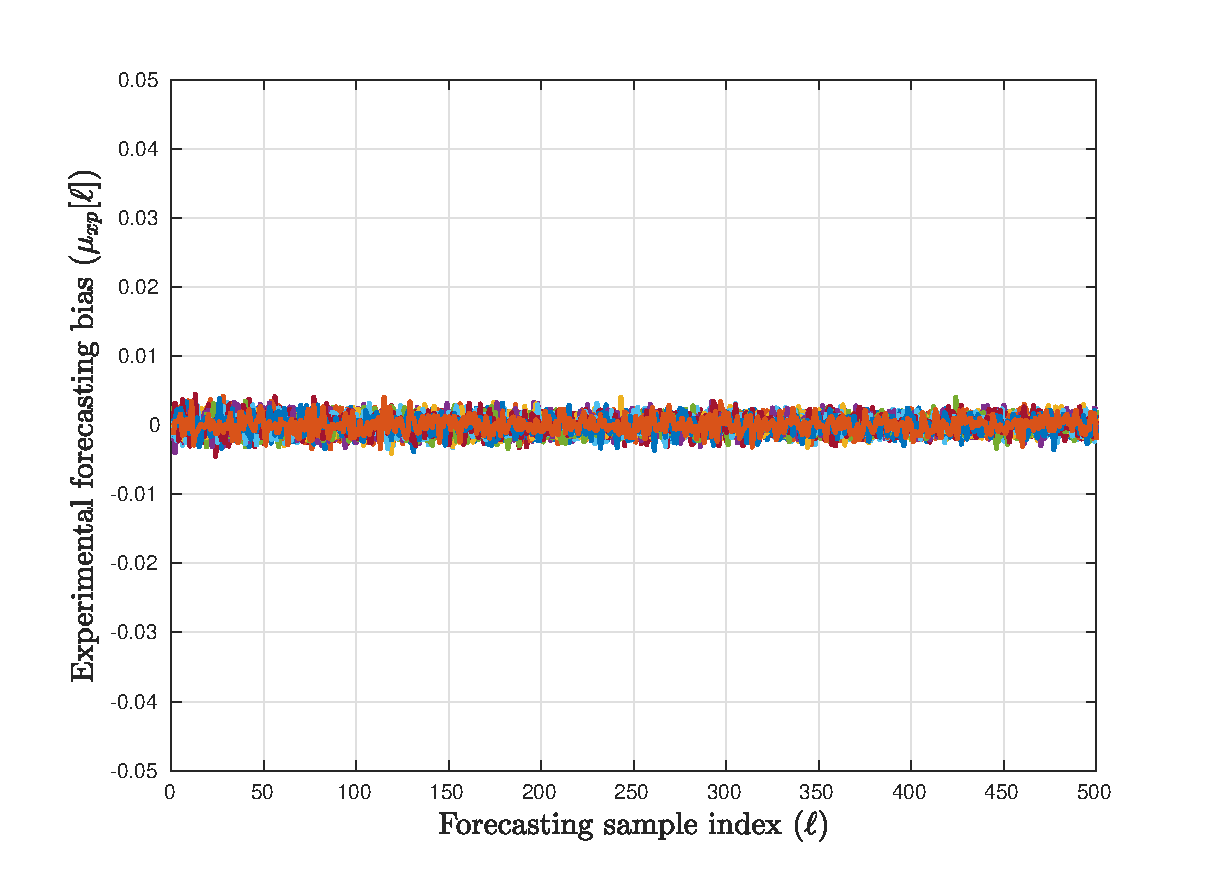
\includegraphics[width=.24\textwidth]{biasNoiseSine.eps}
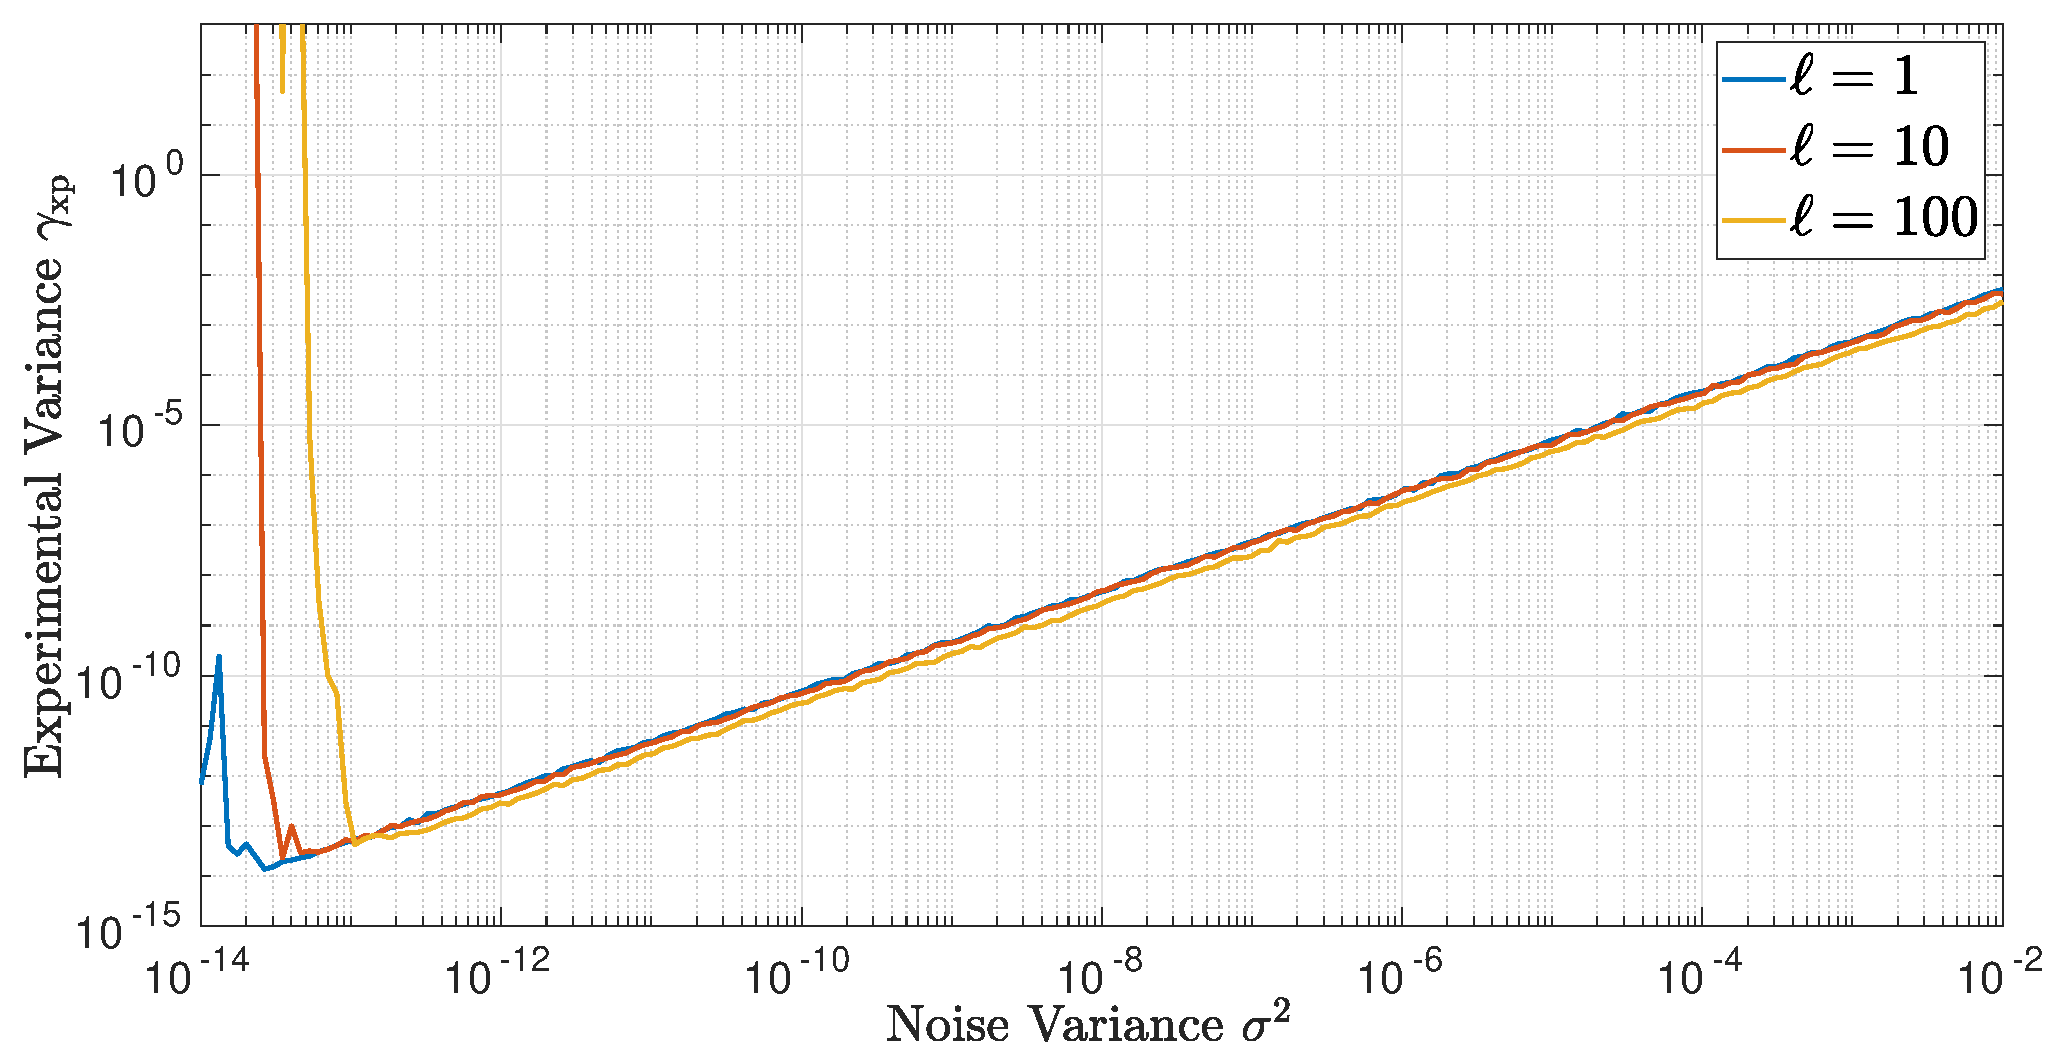
\includegraphics[width=.48\textwidth]{VarianceNoiseSine.eps}
\caption{Evolution of the experimental and theoretical forecasting variance in function of the forecasting sample index for different values of $\sigma$.}
\label{fig:res.noise.sine}
\end{figure}

\paragraph{Influence of the training dataset size $K$} Here, the noise variance $\sigma$ is set to $\sigma=10^{-2}$. Then, the forecasting algorithm is run on 3000 realizations on the discrete signal $\bx$ for three different values of $K$, logarithmically equi-spaced from $4.5\times 10^{2}$ to $2\times 10^{3}$. For each of these values, we determine the experimental bias $\mu_{\xp}[N-1+\ell]$ and variance $\gamma_{\xp}[N-1+\ell,N-1+\ell]$ in function of the forecasting sample index $\ell$ (going from $1$ to $500$). 

As in the previous study, the experimental bias vanishes when $K$ increases, what confirms the approximation result~\eqref{eq:mean.error}. Besides, the experimental variance  is displayed on Fig.~\ref{fig:res.size.sine}, and compared with the associated theoretical variance~\eqref{eq:cov.error.2}. Each color corresponds to these experimental results obtained for a given value of $K$. This result validates the asymptotic behavior provided by~\eqref{eq:cov.error.2}, and we can show that the second order moment $\gamma[\ell,\ell]$ is less dependent on $K$ when $K$ is large.


\begin{figure}
%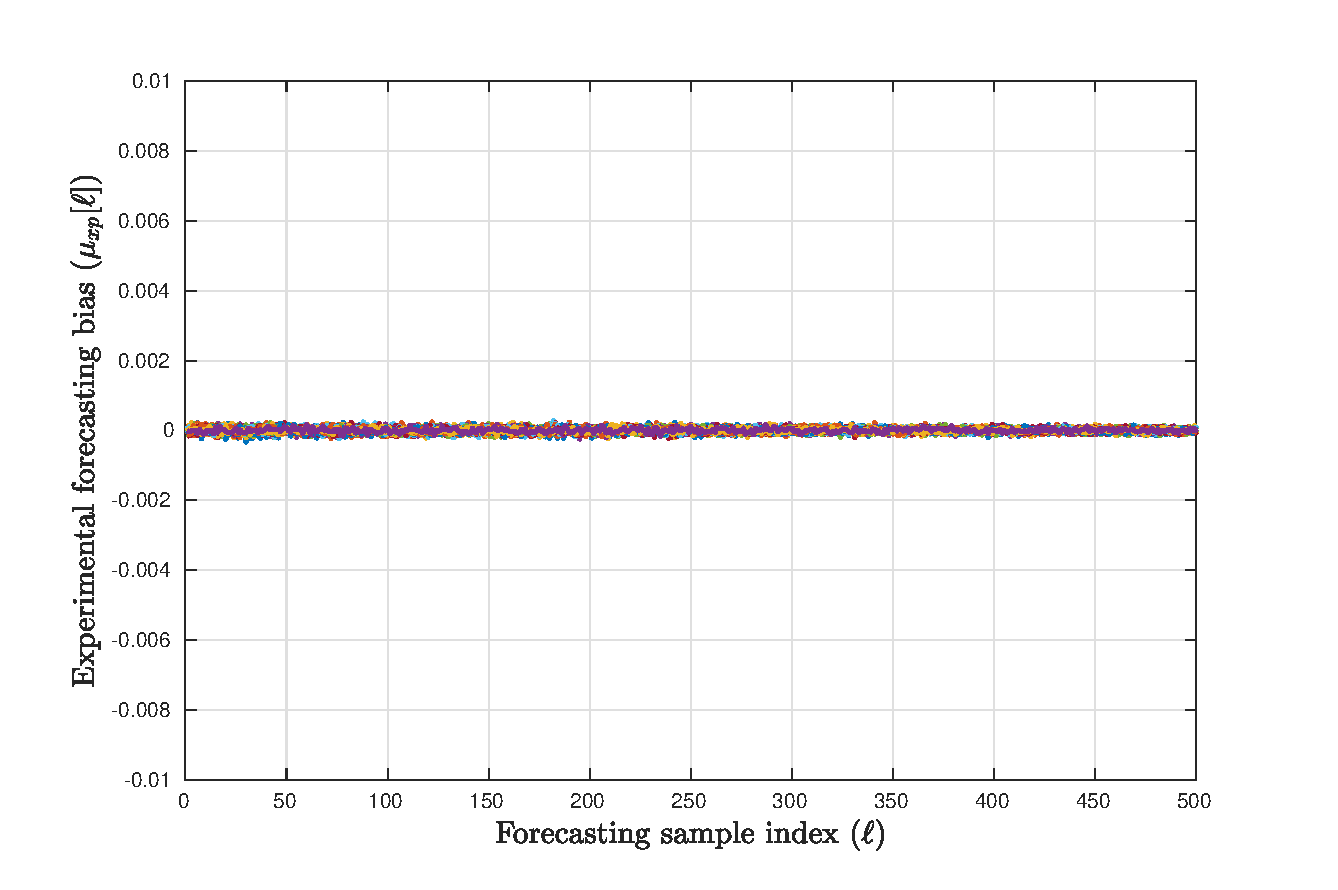
\includegraphics[width=.24\textwidth]{BiasKSine.eps}
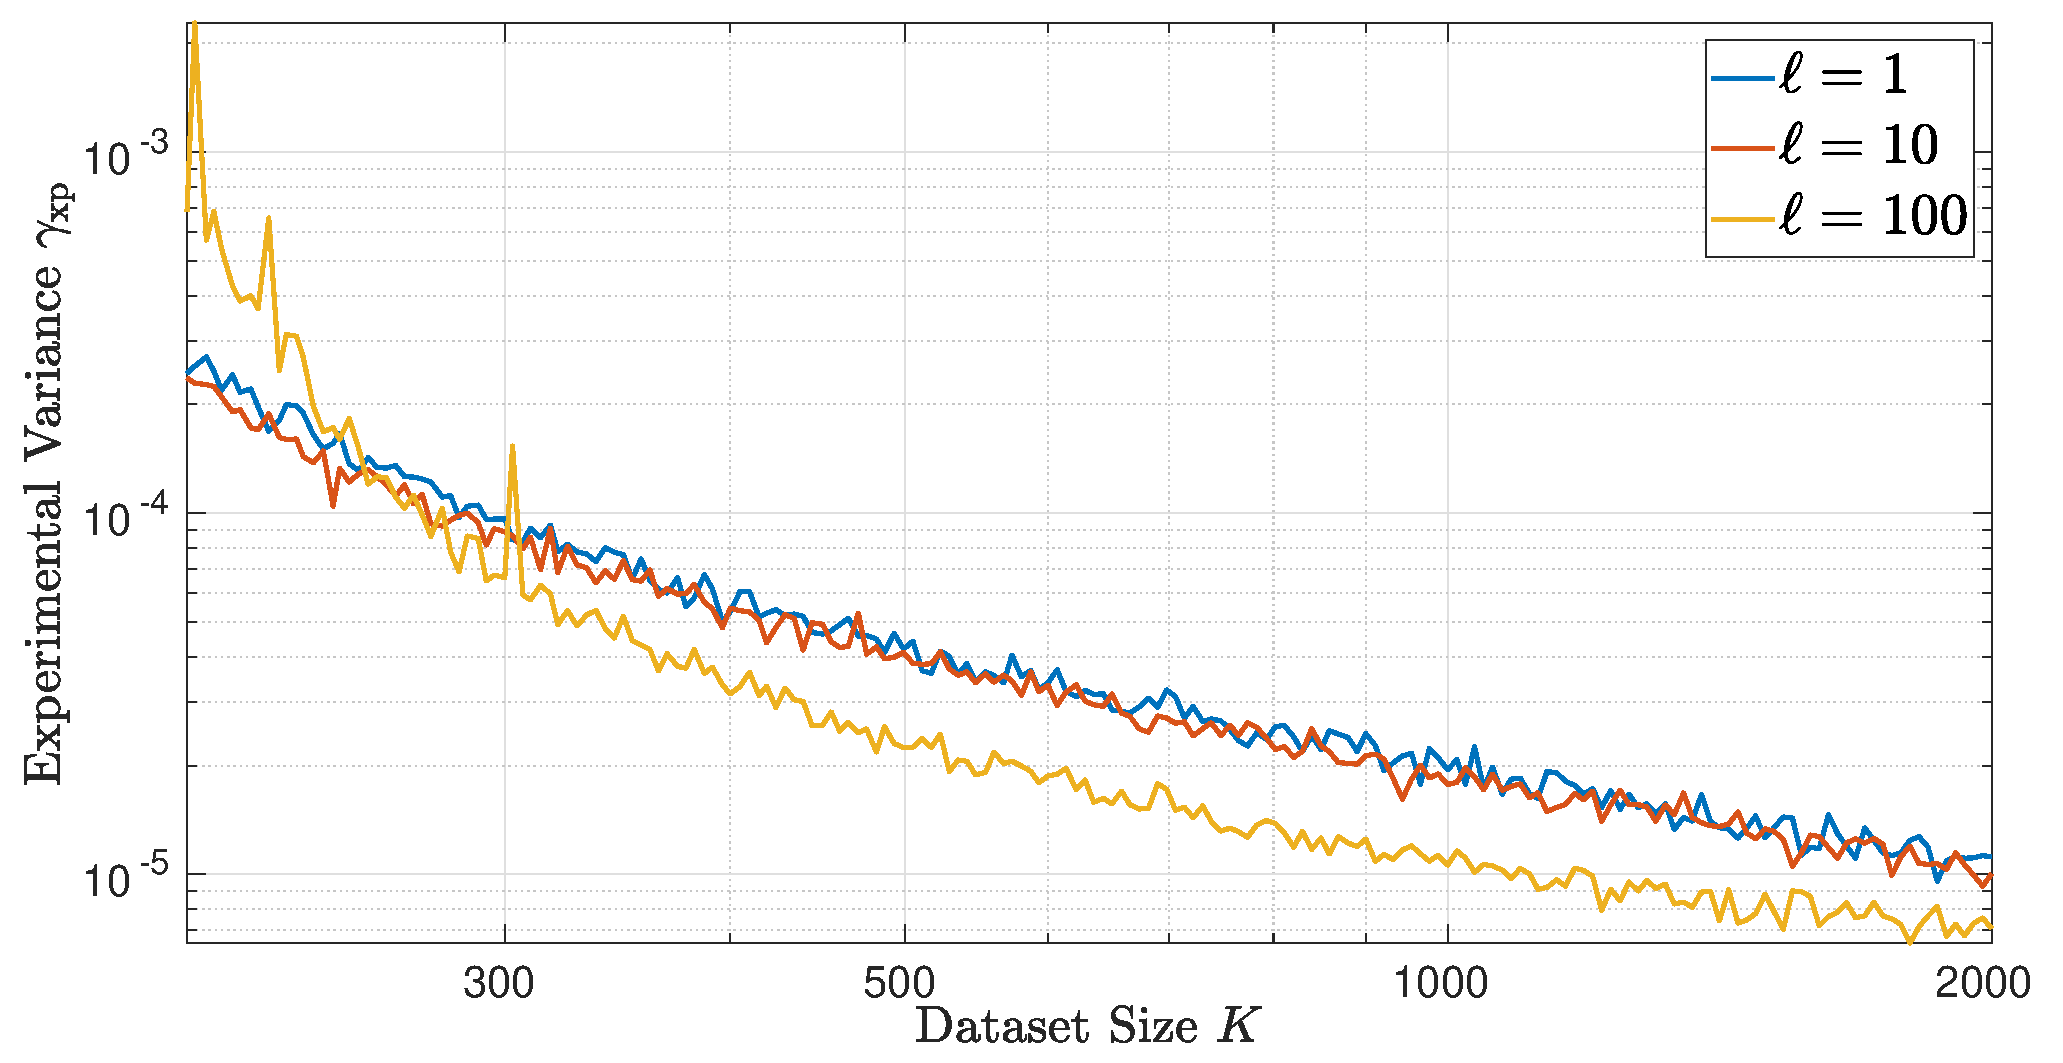
\includegraphics[width=.48\textwidth]{VarianceKSine.eps}
\caption{Evolution of the experimental and theoretical forecasting variance in function of the forecasting sample index for different values of $K$.}
\label{fig:res.size.sine}
\end{figure}

\paragraph{Summary}
Both previous experimental results combined with the theoretical asymptotic equation~\eqref{eq:cov.error.2} allow us to describe the influence of the noise variance and the size of the training dataset on the variance of the forecasting noise, empirically summarized as follows:
\begin{equation}
\gamma[N-1+\ell,N-1+\ell] \underset{K\to\infty}{\approx} \dfrac{\sigma^2}{K}g[\ell] .
\end{equation} 
where $g$ is a bounded positive function. The empirical result is coherent with the theoretical result provided by Theorem~\ref{th:error}.

This study neglects the analysis of the influence of the parameter $M$, whose influence on the value of the experimental variance is numerically not significant as long as $M\ll 2K$. The choice of this parameter is especially crucial when the deterministic component of the signal is no longer stationary. The AHM, discussed below, is an example.

\subsubsection{Adaptive harmonic model}
\label{ssse:res.ahm}
We now consider a signal satisfying the AHM so that the instantaneous frequencies and amplitudes of its components vary over time. The deterministic component $\bz$ of the random vector $\bx$ (constructed following the model~\eqref{eq:model.noise}) takes the following form, for all $n\in\{1,\ldots,N\}$:
\[
\bx[n] = \cos\left(2\pi \phi_1[n] \right) + R[n]\cos\left(2\pi \phi_2[n] \right) \ ,
\] 
where the instantaneous amplitude $R$ is given by:
\[
R[n] = 1.4 + 0.2\cos\left(4\pi\frac{n}{N}\right)\ ,
\]
and the instantaneous phases are such that:
\begin{align*}
\phi_1[n] &= \frac{p_1}{M}\left( n + \frac{0.01}{2\pi}\cos\left(2\pi\frac{n}{N}\right) \right) \\[-1mm]
\phi_2[n] & = p_2\frac{n}{M} + \frac{20}{2N\fs}n^2
\end{align*}
Besides, the noise is chosen to be Gaussian: $\bw\sim\cN(\bzero,\bI)$, and we take: $N=10^4$, $M=750$, $p_1=10$, $p_2=23$.

To highlight the fact that the linear dynamical model is sufficient to catch most of the dynamical behavior of signals following the AHM, we compare the performance of the Algorithm~\ref{alg:boundary} with a simple extension obtained by pointwise symmetrization~\cite{Kharitonenko02wavelet}. We also evaluate the performance of reference forecasting algorithm that could be used for extending such signals. These methods are:
\begin{itemize}
\item The EDMD has been developed by Williams \etal~\cite{Williams15data}. The proposed algorithm is a way to obtain an approximation of the so-called Koopman operator of the observed system, which theoretically allows to catch dynamic of nonlinear systems~\cite{Korda18linear}.
\item The GPR~\cite{Rasmussen06gaussian} is a method relying on a probabilistic dynamical model. That one is based on the Gaussian process structure, and therefore offer more flexibility in the type of dynamic that could be modeled than the linear model~\eqref{eq:dyn.model}.
\item The TBATS method~\cite{DeLivera11forecasting} is based on a classical decomposition of times series into a trend, a seasonal and an ARMA components, with a specific dynamic for the seasonal component. This model demands the estimation of numerous parameters and, by implication, may be slow. 
\end{itemize}

To quantify the global quality (\ie~not depending on $\ell$) of the forecasting approaches, we evaluate the Experimental Mean Square Error $\mathrm{MSE_{xp}}(\tilde\bx)$ of the forward forecast extended signals, namely:
\begin{align}
\label{eq:mse}
\mathrm{MSE_{\xp}}(\tilde\bx) &= \dfrac1{L}\|\tilde\bx -\bx^\mathrm{ext}\|^2 \\[-1mm]
\nonumber
&=\! \dfrac1{L}\sum_{\ell=1}^L \bmu_{\xp}[N\!-\!1\!+\!\ell]^2 \!+\! \bgamma_{\xp}[N\!-\!1\!+\!\ell,N\!-\!1\!+\!\ell] .
\end{align}
where $\bx^\mathrm{ext}$ is the ground-truth extended signal, that is: $\bx^\mathrm{ext} = \begin{pmatrix}\bx[-L] & \cdots & \bx[N-1+L] \end{pmatrix}$. Then, as long as the bias $\bmu[N-1+\ell]$ and the variance $\bgamma[N-1+\ell,N-1+\ell]$ of the forecasting estimator remain small for all $\ell$, the MSE takes small values either. Corresponding results are given in Table~\ref{tab:mse.sine}. They show that the naive extension we propose gives satisfying results, in particular in comparison with the point-symmetric extension. Besides, even though the other more sophisticated methods, like GPR, give MSE values that have a slightly smaller standard deviation, these methods are substantially limited by the computing time they require, which prevent them from being used to exploit real-time data. Thus, {\sf SigExt} is the extension method that optimize the trade-off between the forecasting quality and the computing time. %That is why, it is implemented in our algorithm for the reduction of boundary effects.

\begin{table}
\centering
\caption{AHM signal. Performance of the extension methods.}
\begin{tabular}{|c||c|c|c|}
  \hline
   \multirow{2}{*}{Algorithm} & \multicolumn{2}{c|}{MSE}  & \multirow{2}{41pt}{Computing time (sec.)} \\
   \cline{2-3} & Mean & Standard deviation & \\
   \hhline{|=#=|=|=|}
   {\sf SigExt} & $1.433\times 10^{-3}$ & $4.361\times 10^{-4}$ & $0.152$ \\
   \hline
   Symmetric & $1.019\times 10^{1}$ & $1.192\times 10^{2}$ & $0.002$ \\
   \hline
   EDMD & $3.076\times 10^{-2}$ & $8.095\times 10^{-2}$ & $2.537$\\
   \hline
   GPR & $1.436\times 10^{-3}$ & $4.346\times 10^{-4}$ & $146.331$ \\
   \hline
   TBATS & $1.732\times 10^{-3}$ & $4.924\times 10^{-4}$ & $1837.120$ \\
   \hline
\end{tabular}
\label{tab:mse.sine}
\end{table} 


\subsection{Evaluation of the quality of the boundary effects reduction}

\subsubsection{Metrics}
The quality of the boundary effects reduction is evaluated directly on the TF representation. To that aim, we compare the obtained representation to the optimal representation $\ccF_N^\mathrm{opt}(\bx)$, defined as the restriction of the representation of the ground-truth extended signal $\bx^\mathrm{ext}$. Therefore, we have:
\begin{equation}
\ccF^\mathrm{opt}(\bx_N) = \cR\left( \ccF(\bx^\mathrm{ext}) \right) \ .
\label{eq:opt.TFR}
\end{equation} 

In the aim of comparing the different techniques, we use a criterion, proposed in~\cite{Daubechies16conceft}, that quantify the distance between a given TF representation and the optimal one. It is built in analogy with the optimal transport distance, which enables quantifying the distance between two probability density functions. Let us generically denote a time frequency representation $\ccQ$. Then, for $t$ fixed, we consider the following probability density function: $p_\ccQ^t(\xi) = \left. |\ccQ(\xi,t)|^2 \middle/ \int_\RR |\ccQ(\nu,t)|^2\dd\nu \right.$. At each instant $t$, we can then determine the optimal transport distance $d_{t}$ between the two densities. It is given by the $L^1$ norm of the difference between the associated distribution functions. In other words, we have:
\begin{equation*}
d_{t}(\ccQ,\ccF_0) = \int_\RR\left|\tilde P_{\ccQ}^t(\xi)-  P_{\ccF_0}^t(\xi)\right|\dd\xi\ ,
\end{equation*}
where $P_{\ccQ}^t(\xi)=\int_{-\infty}^\xi p_{\ccQ}^t(\nu)\dd\nu$ and $\tilde P_{\ccF_0}^t(\xi)=\int_{-\infty}^\xi\tilde p_{\ccF_0}^t(\nu)\dd\nu$. The \textit{optimal transport distance} quantifies the proximity between the estimated and actual instantaneous frequencies while favoring the sparsity of the estimated TF representation. That is why, the performance index $D(\ccQ)$ for the reduction of boundary effects of a given TF representation $\ccQ$ is given by the averaged ratio between the optimal transport distance to the optimal TF representation~\eqref{eq:opt.TFR} and the optimal transport distance of to the optimal TF representation, that is:
\begin{equation}
D(\ccQ) = \dfrac1{|I|}\bigintss_I\ \frac{d_{t}\left(\ccQ,\ccF^\mathrm{opt}\right)}{d_{t}\left(\ccF,\ccF^\mathrm{opt}\right)}\ \dd t\ .
\label{eq:index.perf}
\end{equation}
Thus, $D(\ccQ)<1$ means a reduction of the boundary effects. Let us evaluate the quality of the boundary effects reduction on biomedical signals.


\subsubsection{Respiratory signal}
We first consider a respiratory signal of 6 hours 20 minutes. This signal, a small portion of which is displayed in Fig.~\ref{fig:tho}, is sampled at $\fs=100$~Hz.

\begin{figure}
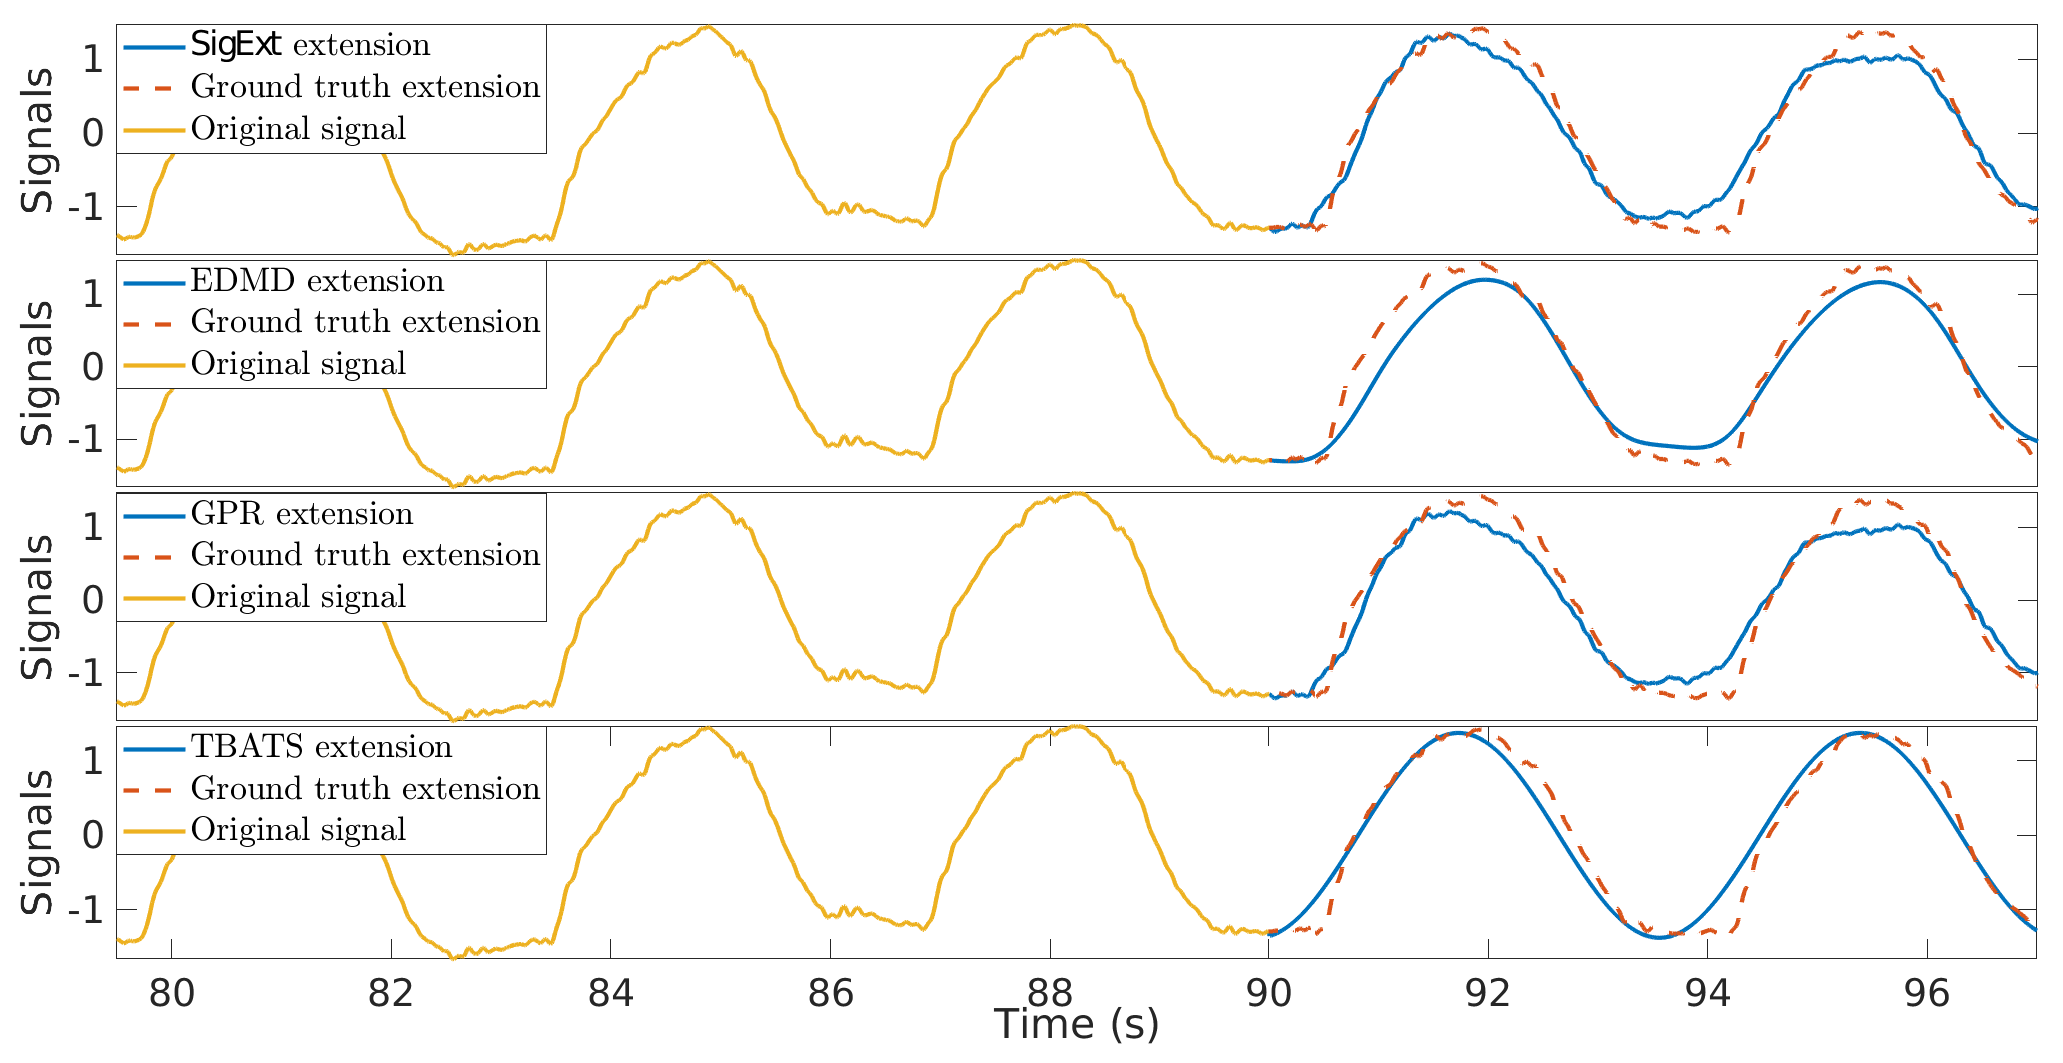
\includegraphics[width=.48\textwidth]{THOforecast.eps}
\caption{Extended THO signal (blue) obtained by the {\sf SigExt} forecasting (top), the EDMD forecasting (middle), and the GPR forecasting (bottom), superimposed with the ground truth signal (red dash).}
\label{fig:tho}
\end{figure}

From that large signal, we build a dataset of $378$ non-overlapping signals of 60 seconds, \ie~$N=6000$. On each of these pieces of signal, we implement the forecasting method introduced in section~\ref{ssse:res.ahm}, including the {\sf SigExt} method detailed in Algorithm~\ref{alg:extension}. However, the TBATS extension method in not implemented here because of its excessive computing time. The extensions of $7$ seconds-long on each boundary, corresponding to $L =700$. Thus, in order to catch slowly varying dynamical behaviors, the size of the training signal $M$ is chosen so that $M=\lfloor 1.5L\rfloor$. As a result of section~\ref{ssse:res.sine}, we take: $K=\lfloor2.5M\rfloor$. The resulting MSE~\eqref{eq:mse} averaged with respect to the simulations are given in Table~\ref{tab:THO}. The MSE of {\sf SigExt} is higher than the MSE of the other methods. This is mainly caused by the presence of a few segments of the whole signal involving complicated behaviors, that are unpredictable via a too simple dynamical model like~\eqref{eq:dyn.model}. The left of Fig.~\ref{fig:THO.failure} illustrates one of those cases, where {\sf SigExt} fails to catch the fast varying dynamic of the instantaneous amplitude to satisfactorily forecast the signal. The EDMD an Symmetric extensions are more robust to those situations, as shown on this example and in Table~\ref{tab:THO}. Nevertheless, {\sf SigExt} provides a sufficiently relevant extension to give TF representations sparingly affected by boundary effects. On the right of Fig.~\ref{fig:THO.failure}, we display comparison between the right boundary of SST of the same segment of signal (top-right), and its boundary-free SST obtained after the {\sf SigExt} forecasting (bottom-right). The extension of the instantaneous frequency visible on the right side of the image, illustrates the reduction of boundary effects produced despite an inaccurate signal forecasting.

We then apply {\sf BoundEffRed} (\ie~Algorithm~\ref{alg:boundary}) for diverse TF representations: STFT, SST, RS, as well as concentration of frequency and time (ConceFT), a generalized multitaper SST-based representation introduced in~\cite{Daubechies16conceft}. In Table~\ref{tab:THO}, we give the averaged performance index~\eqref{eq:index.perf}, evaluated the whole TF representations (including  boundaries). Even though {\sf SigExt} performs somehow moderately, the boundary effects are dramatically reduced on the TF representations, in the same order of magnitude than with the forecastings given by EDMD or GPR. Notice that the extension length $L$ has been set accordingly to the window length used by the TF analysis tool. For instance, the window length used to evaluate the STFT is of $1500$ samples. To prevent the STFT from being sensitive to the boundaries, we set $L=750$. In this way, the evaluation of the spectral content of the signal near its boundaries is not limited by a lack of information all along the window support. From now on, all results are given for $L$ equal to the half of the width of the window used in the TF transform.

\begin{table}
\centering
\caption{Performance of the extension methods on a respiratory signal.}
\begin{tabular}{|c||c||c|c|c|c|}
  \hline
   \multirow{2}{*}{Algorithm} & \multirow{2}{35pt}{\centering Averaged MSE} & \multicolumn{4}{c|}{Averaged performance index $D$} \\
   \cline{3-6}
      & & STFT & SST & RS & ConceFT \\
   \hhline{|=#=#=|=|=|=|}
   {\sf SigExt} & $0.046$ & $0.705$ & $0.698$ & $0.694$ & $0.776$ \\
   \hline
   Symmetric & $0.039$ & $1.280$ & $0.984$ & $9.063$ & $1.295$ \\
   \hline
   EDMD & $0.022$ & $0.757$ & $0.635$ & $0.701$ & $0.793$ \\
   \hline
   GPR & $0.045$ & $0.817$ & $0.793$ & $0.727$ & $0.876$ \\ 
   \hline
\end{tabular}
\label{tab:THO}
\end{table}

\begin{figure}
\centering
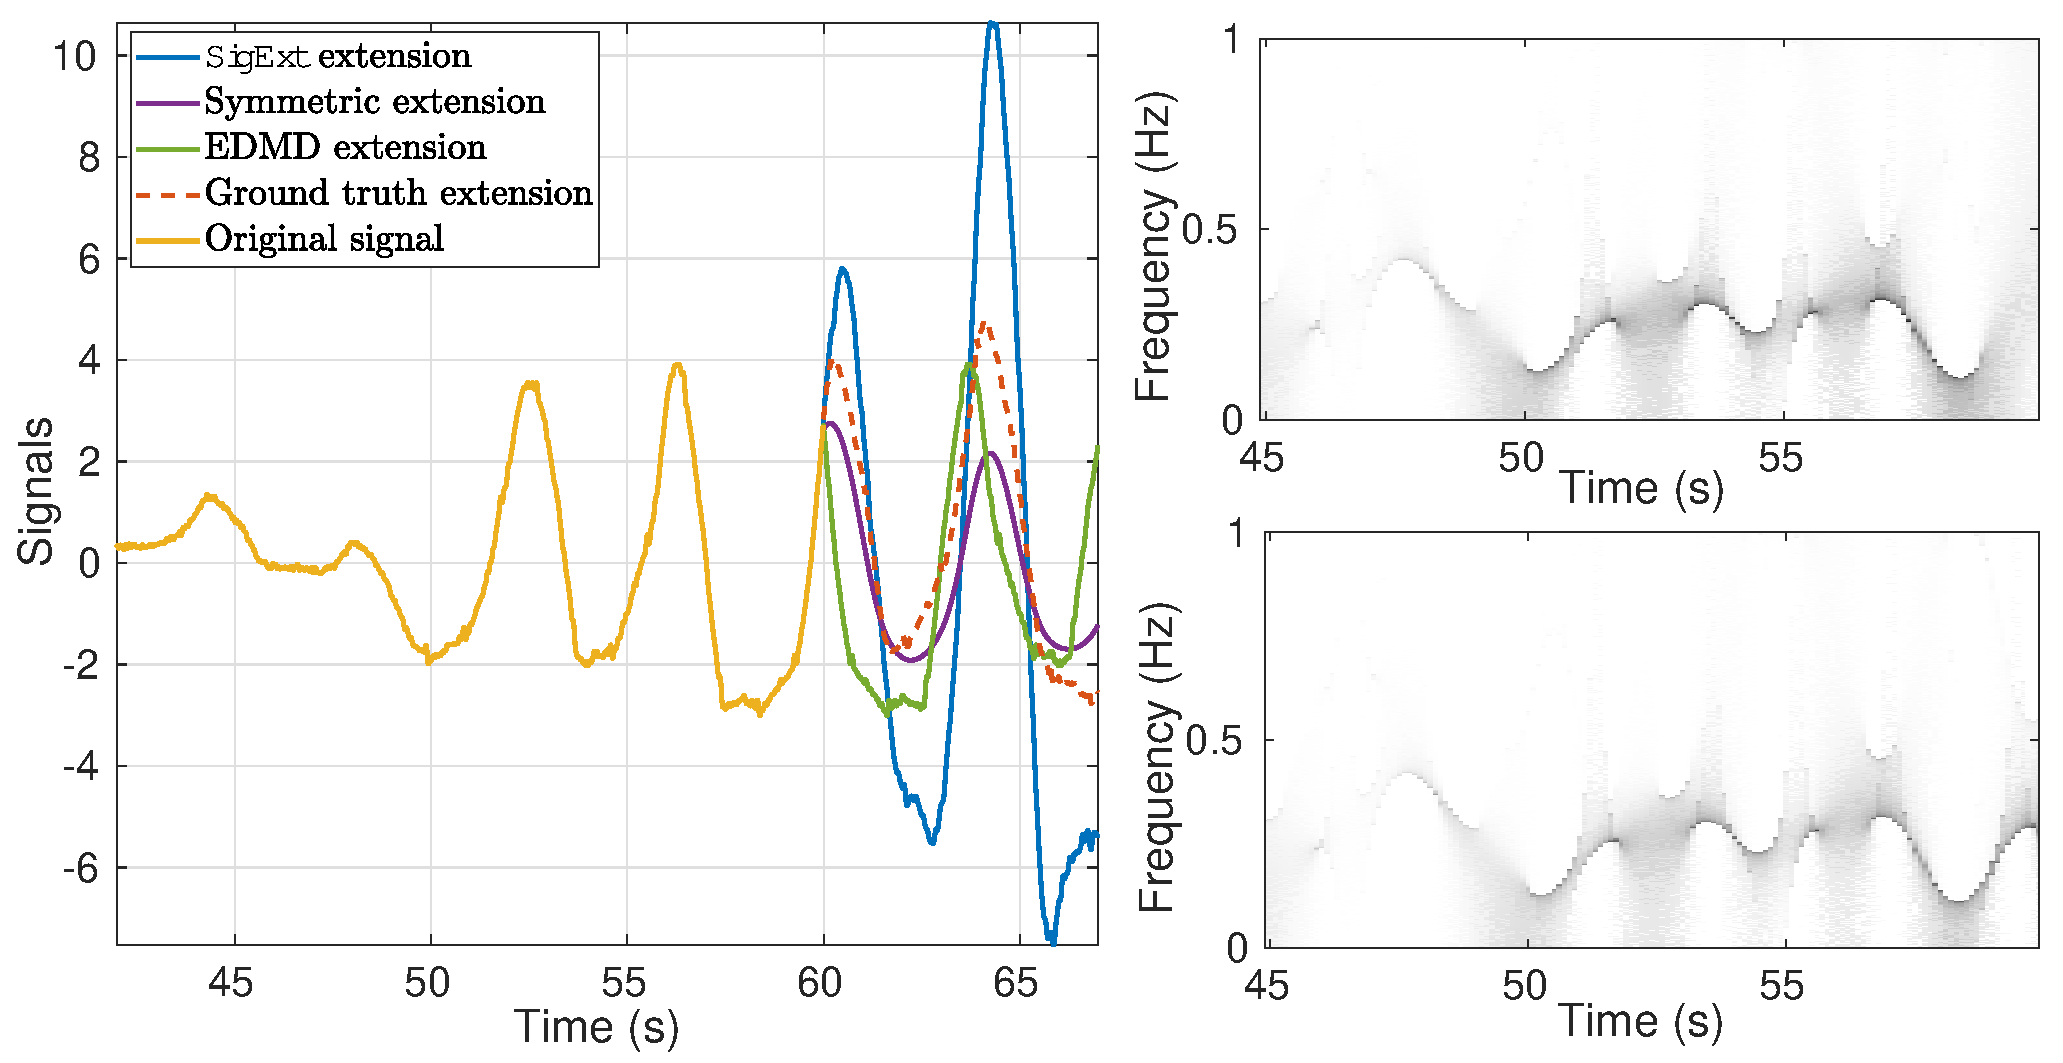
\includegraphics[width=.48\textwidth]{THOfailure.eps}
\caption{Extensions of a segment of the respiratory signal (left) where {\sf SigExt} is outperformed by the EDMD and Symmetric extensions. Corresponding SST (top-right) and boundary-free SST obtained with {\sf SigExt} (bottom-right).}
\label{fig:THO.failure}
\end{figure} 

Finally, in order to verify the ability of {\sf BoundEffRed} to be implemented in real time, we evaluate the computation time required for each iteration of Algorithm~\ref{alg:boundary}, corresponding to the update of the boundary-free TF representation. This check is performed on the real-time SST of a 10-minute sample of the respiratory signal. As the SST is temporally sub-sampled by a ratio of 10, the update should not exceed $10/\fs=0.1$~sec. This is indeed the case, as no iteration lasted longer than xx sec on a 6-Core Xeon CPU running at 3.5~GHz and 64~GB of RAM.


\subsubsection{Photoplethysmogram}
\label{ssse:ppg}
We perform a study similar to the previous one on a 640 second-long photoplethysmogram (PPG) signal extracted from the Physionet dataset~\cite{Pimentel17toward, Goldberger00physiobank}, sampled at $\fs=125$~Hz. A 32 second-long piece of this signal is displayed on the top of Fig.~\ref{fig:ppg}. The estimated 2-second extension obtained by {\sf SigExt} on both boundary of this signal is superimposed to the ground-truth signal in the bottom of Fig.~\ref{fig:ppg}.

\begin{figure}
%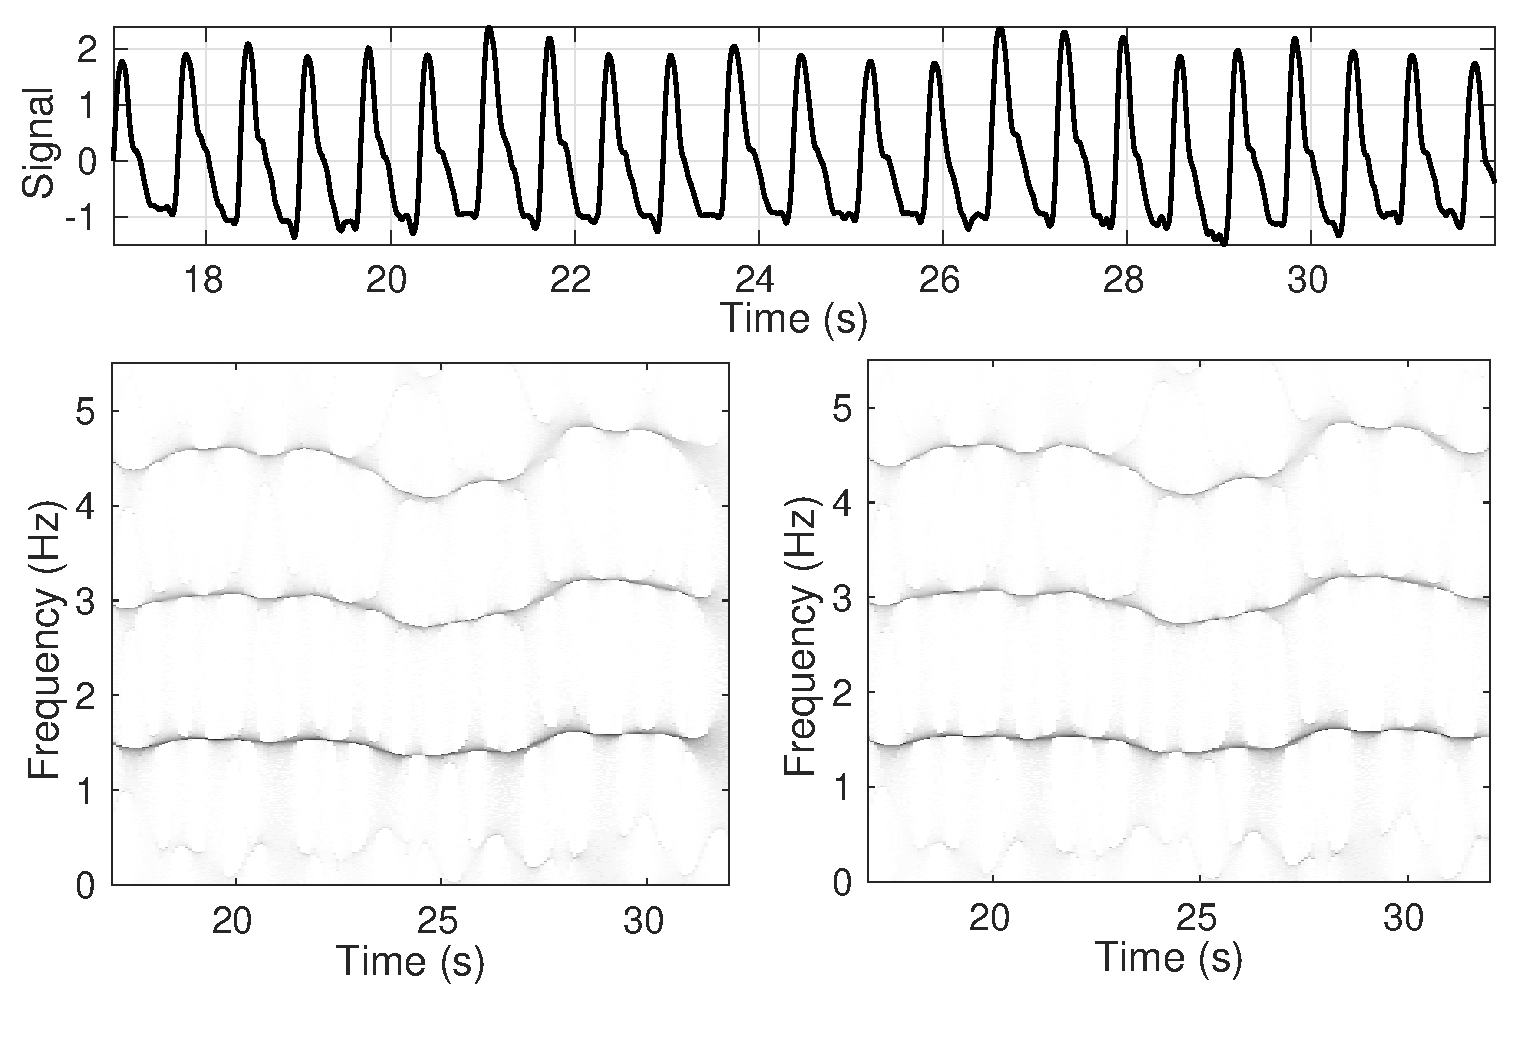
\includegraphics[width=.48\textwidth]{PPGsig.eps}
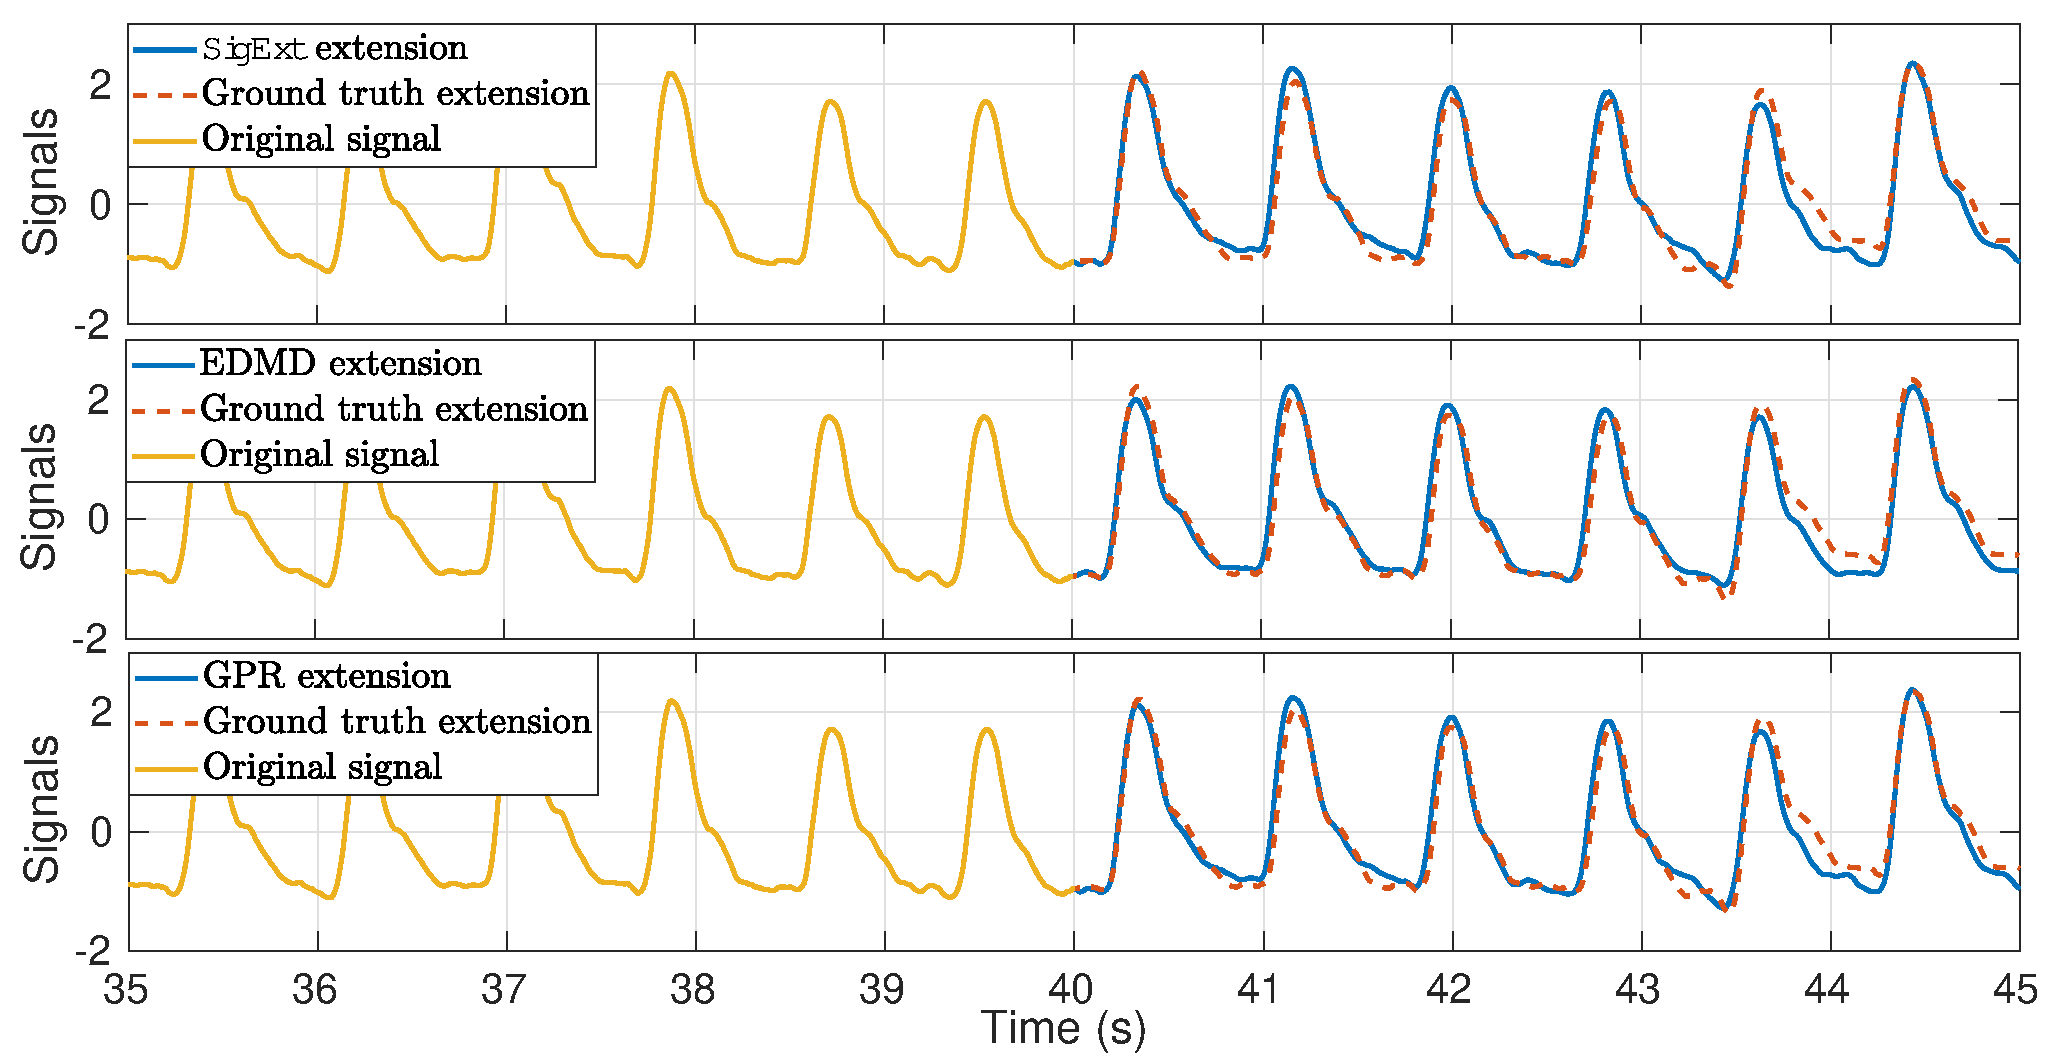
\includegraphics[width=.48\textwidth]{PPGforecast.eps}
\caption{Extended PPG signal (blue) obtained by the {\sf SigExt} forecasting (top), the EDMD forecasting (middle), and the GPR forecasting (bottom), superimposed with the ground truth signal (red dash).}
\label{fig:ppg}
\end{figure}

We divide the signal into 32-second long segments, and apply Algorithm~\ref{alg:boundary} on each piece. We provide in Table~\ref{tab:otd.ppg} the performance index $D$ of the boundary-free TF representations averaged over the signals. For all the considered TF representations, the results clearly shows that our algorithm reduces the boundary effects. %This highlights the ability of our approach to limit the distortion due the boundary effects and provide a more accurate representations. 
Even though, on this signal, the {\sf SigExt} extension yields TF representations slightly more sensitive to boundary effects than the extensions given by EDMD or GPR, it is the only technique that allows a real-time implementation.

\begin{table}
\centering
\caption{PPG signal: averaged performance index of the boundary-free TF representations for different extensions.}
\begin{tabular}{|c||c|c|c|}
  \hline
   \multirow{2}{*}{Extension method} & \multicolumn{3}{c|}{Performance index $D$} \\
   \cline{2-4}
      & STFT & SST & ConceFT\\
   \hhline{|=#=|=|=|}
%   Without extension & $2.52\times 10^{-2}$ & $9.41\times 10^{-2}$ & $1.03\times 10^{-1}$ \\
%   \hline
   {\sf SigExt} & $0.774$ & $0.048$ & $X$ \\
   \hline
   Symmetric & $0.818$ & $0.059$ & $X$ \\
   \hline
   EDMD & $0.566$ & $0.038$ & $X$ \\
   \hline
   GPR & $0.735$ & $0.045$ & $X$ \\
   \hline
\end{tabular}
\label{tab:otd.ppg}
\end{table}

On the bottom-right panel of Fig.~\ref{fig:ex.intro}, we display the SST resulting from the {\sf BoundEffRed} strategy, applied to the portion of PPG displayed on Fig.~\ref{fig:ppg}. We clearly observe an improvement of the quality of the SST near boundaries. Indeed, the blurring visible when zooming on the right boundary of the SST has almost vanished. The real-time tracking of the instantaneous frequencies contained in the measured signal is therefore largely facilitated.

%\begin{figure}
%\centering
%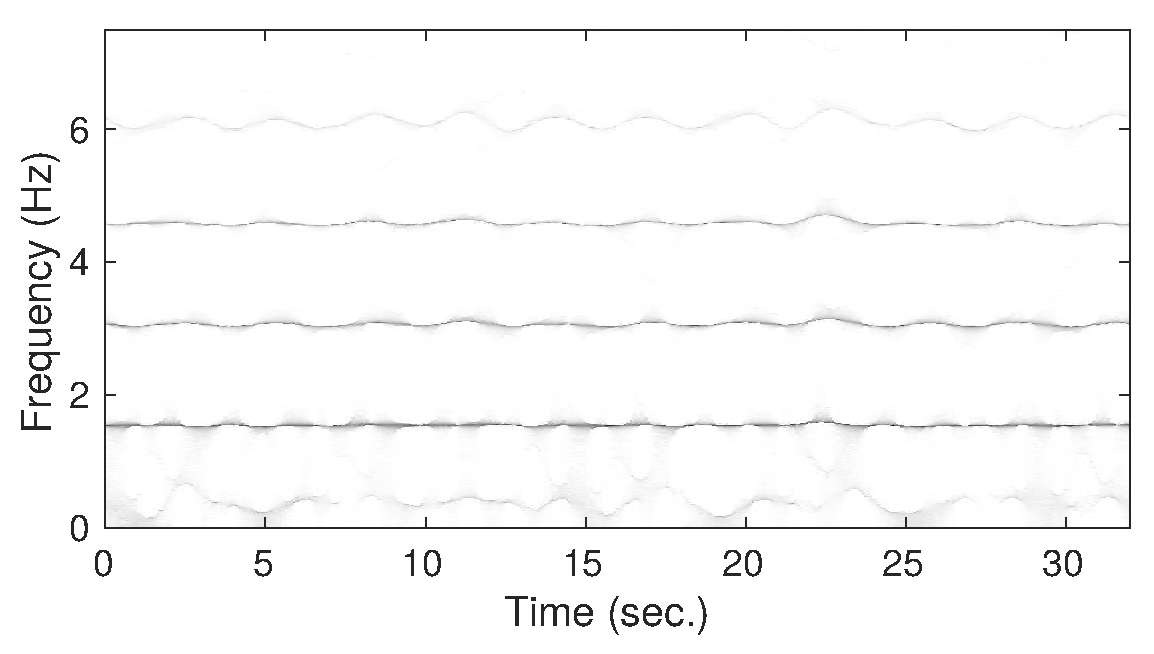
\includegraphics[width=.48\textwidth]{SSTBoundEffRed.eps}
%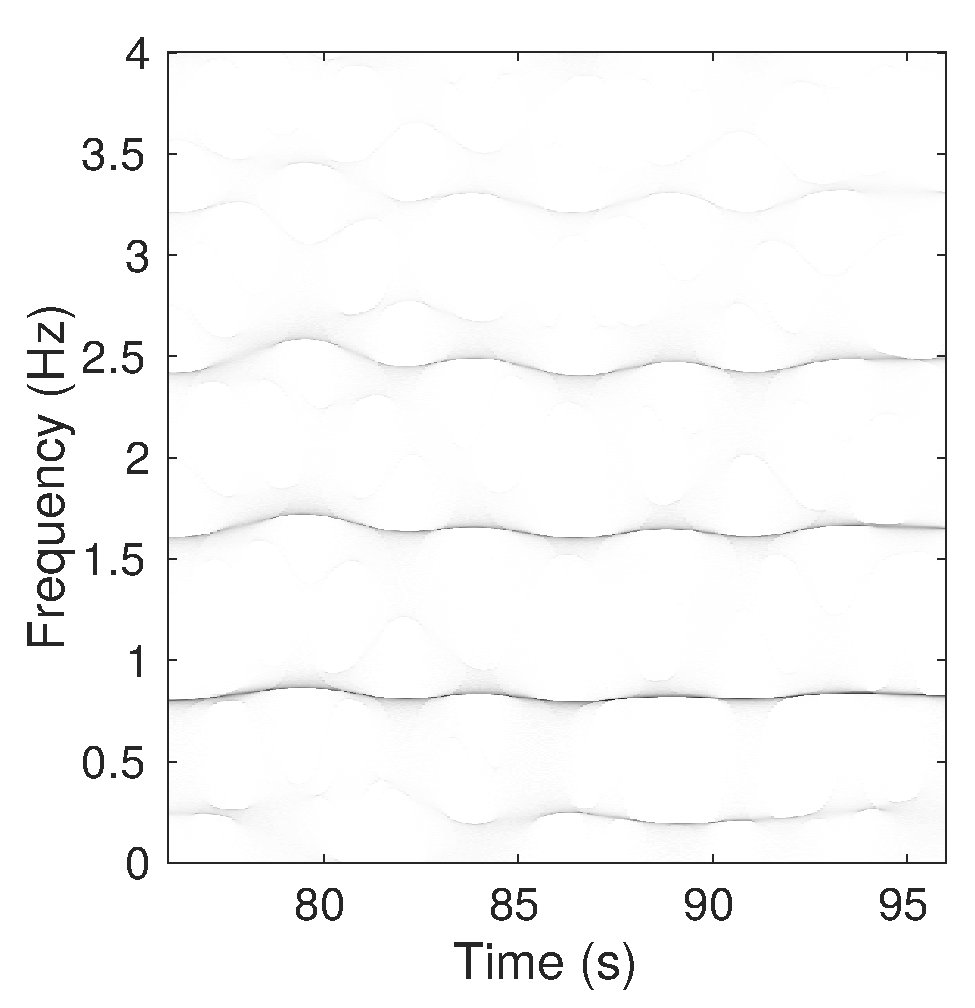
\includegraphics[width=.48\textwidth]{zoomSSTBoundEffRed.eps}
%\caption{Result of {\sf BoundEffRed} on the synchrosqueezing transform of a PPG (top) with a zoom on its right boundary (bottom). }
%\label{fig:ppg.boundeffred}
%\end{figure}


To evaluate the influence of the noise level on the performance of {\sf BoundEffRed}, we artificially add a Gaussian noise to the measured PPG signal. It is thus an additional noise to the measurement noise actually contained in the signal. Fig.~\ref{fig:otd.noise} shows the averaged OTD of {\sf BoundEffRed} for different values of the Signal to Noise Ratio (SNR). We notice that STFT is slightly more sensitive to noise than SST or RS, and STFT performs the best when the added noise is small, \ie~when the SNR is great. %On one hand, the robustness to noise of the SST and the RS is the direct consequence of the approximation result of~\cite{Daubechies16conceft}, discussed in section~\ref{sse:perf.BoundEffRed}. On the other hand, the sensitivity to noise of the STFT may be interpreted as the inability to forecast the values of the TF coefficients where only noise is active, while sharp TF representations, such as SST or RS, ideally vanish at these points.


\begin{figure}
\centering
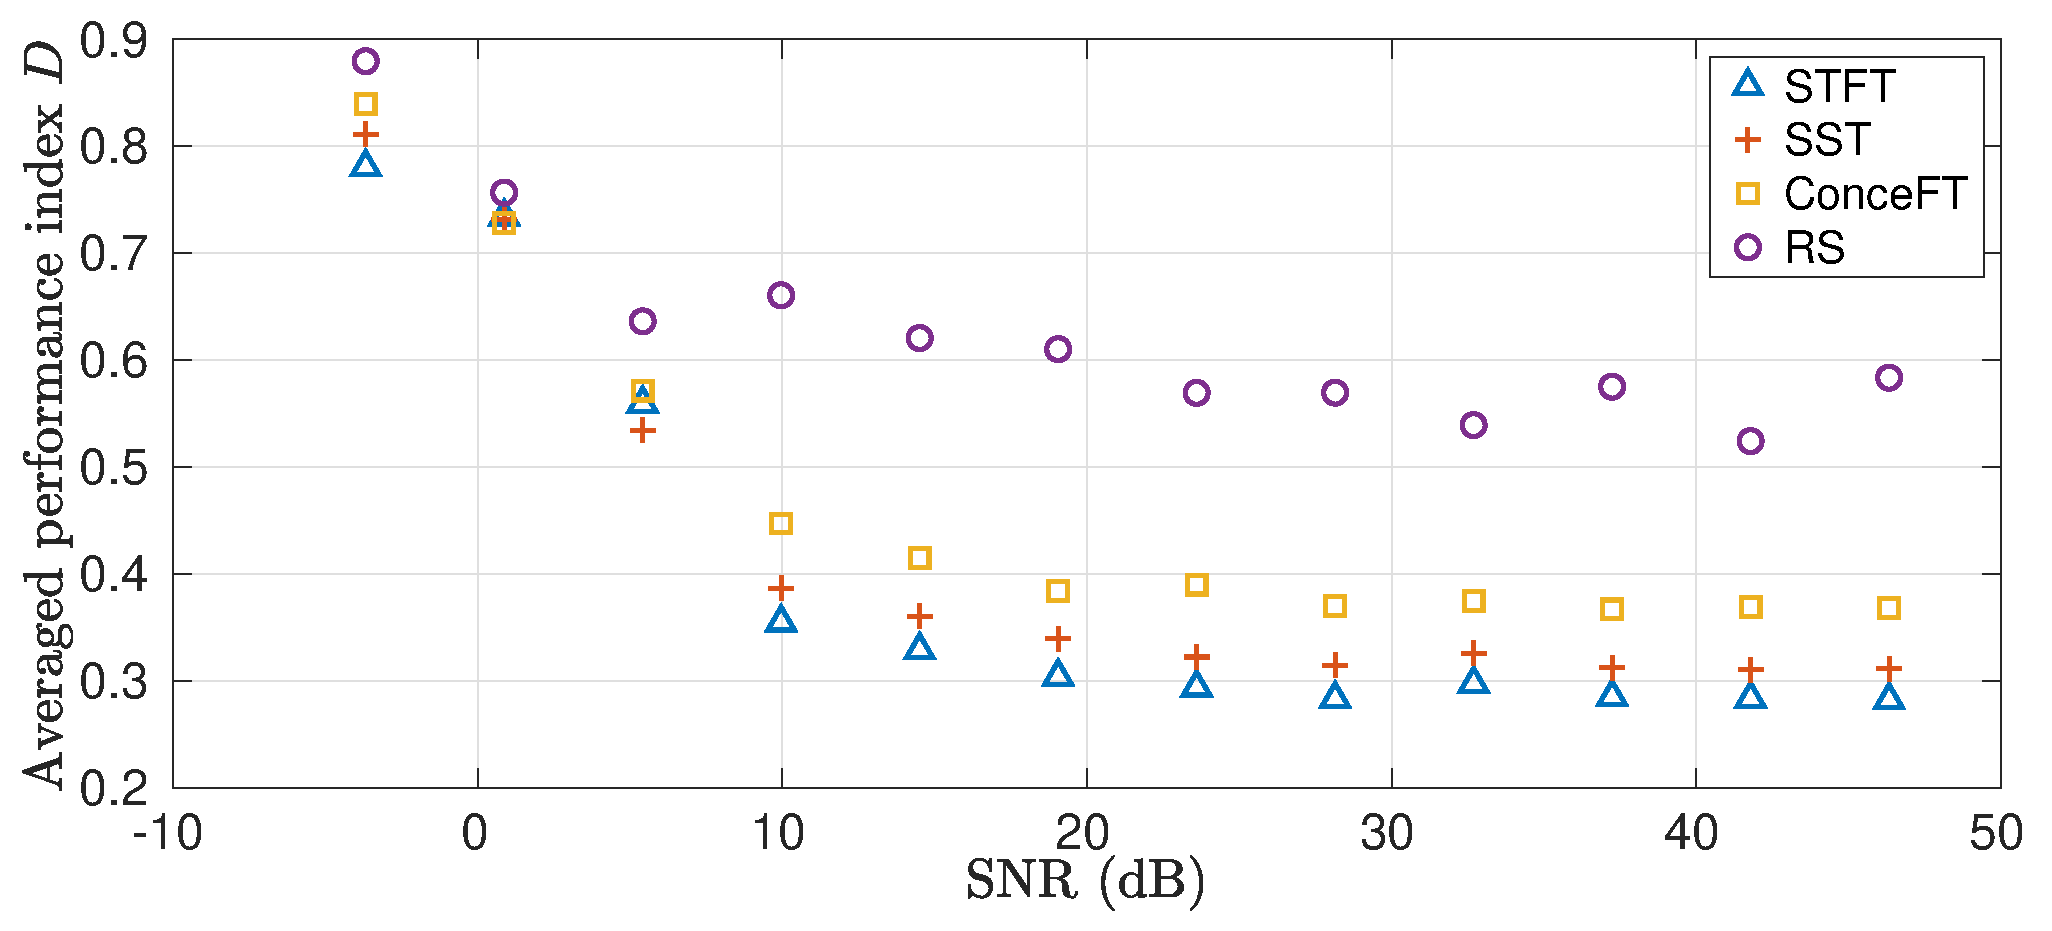
\includegraphics[width=.48\textwidth]{OTDBoundEffRed.eps}
\caption{PPG signal. Averaged OTD of {\sf BoundEffRed} in function of the SNR.}
\label{fig:otd.noise}
\end{figure} 

\section{Conclusion}
\label{se:conclusion}
In this paper, we propose an algorithm, named {\sf BoundEffRed}, for the real-time reduction of boundary effects in TF representations. This method is based on an extension of the signal obtained by a simple-minded and numerically efficient forecasting. We have shown theoretically that the chosen dynamic model is sufficient to extend signals formed by a sum of sine waves. Moreover, the low computational time allows us to switch to a real-time implementation of {\sf BoundEffRed}, unlike other existing forecasting methods. The numerical results also confirmed the robustness to noise of {\sf BoundEffRed}, as well as its ability to be applied to many TF representations. An additional applications to ECG is included in the Supplementary Materials.

Various improvements can be considered to make the algorithm more robust. In particular, we have noticed (see Fig.~\ref{fig:THO.failure}) that when the regular oscillations of the observed signal break, the forecasting step is no longer relevant, and only slows down the calculation of the TF representation. A preliminary step should then be added to the algorithm to detect signal activity and disable the forecasting step when possible. More fundamentally, one can also consider accelerating the computational time by optimizing the forecasting step to improve the real-time performance of {\sf BoundEffRed}. Indeed, each new forecast requires the inversion of the matrix $\bX\bX^T$ of size $M\times M$. However, the matrix $\bX$ used to forecast $\bx_{N+H}$ at the current iteration differs from the one used at the previous iteration to forecast $\bx_{N}$ by only $H$ columns. It then seems natural to take inspiration from the work of Strobach~\cite{Strobach97square}, generalized by Badeau \etal~\cite{Badeau04sliding}, which proposes a fast algorithm for the singular value decomposition of successive data matrices taking the same form as $\bX$. Their algorithm is limited to the case where $H=1$. Developing an extension of this algorithm to variations of $H>1$ columns would then allow us to efficiently update the matrix $\left(\bX\bX^T\right)^{-1}$. These avenues will be explored in our future work.

%\appendices
%\input{appendices}

%\section*{Acknowledgment}

\bibliographystyle{IEEEtran}
\bibliography{AM041320}

%\begin{IEEEbiography}{Michael Shell}
%Biography text here.
%\end{IEEEbiography}
%
%\begin{IEEEbiographynophoto}{John Doe}
%Biography text here.
%\end{IEEEbiographynophoto}


\end{document}